\documentclass[12pt]{article} %openany
\usepackage{fullpage}
\usepackage[affil-it]{authblk}
\usepackage[english]{babel}
\usepackage{graphicx}
\usepackage{rotating}
%\usepackage{bibtex}
%\usepackage[utf8]{inputenc}
%\usepackage[english]{babel}
\usepackage{adjustbox}
\usepackage{courier}
\usepackage{verbatim}
\usepackage{url}
\usepackage[hidelinks]{hyperref}
\usepackage{float}
\usepackage{array}
\usepackage{breakcites}
\usepackage{gensymb}
%\usepackage[backend=biber]{biblatex}
\usepackage{multirow} 
\usepackage{placeins}
\usepackage{booktabs}
\usepackage{tabularx}
\newcolumntype{b}{>{\hsize=1.0\hsize}X}
\newcolumntype{s}{>{\hsize=.5\hsize}X}
\newcolumntype{m}{>{\hsize=.75\hsize}X}
\newcolumntype{x}{>{\hsize=.25\hsize}X}
\newcolumntype{a}{>{\hsize=.11\hsize}X}
\graphicspath{{figures/}}
\usepackage{listings}
\usepackage{appendix}
\usepackage{cite}
\usepackage{blindtext}
\usepackage[utf8]{inputenc} % Required for inputting international characters
\usepackage[T1]{fontenc} % Output font encoding for international characters
\usepackage{mathpazo} % Palatino font
\usepackage{graphicx} % For the logo
\usepackage[acronym,toc]{glossaries}
%\newacronym{<++>}{<++>}{<++>}
\newacronym[longplural={metric tons of heavy metal}]{MTHM}{MTHM}{metric ton of heavy metal}
\newacronym{ABM}{ABM}{agent-based modeling}
\newacronym{ACDIS}{ACDIS}{Program in Arms Control \& Domestic and International Security}
\newacronym{AHTR}{AHTR}{Advanced High Temperature Reactor}
\newacronym{ANDRA}{ANDRA}{Agence Nationale pour la gestion des D\'echets RAdioactifs, the French National Agency for Radioactive Waste Management}
\newacronym{ANL}{ANL}{Argonne National Laboratory}
\newacronym{ANS}{ANS}{American Nuclear Society}
\newacronym{API}{API}{application programming interface}
\newacronym{ARE}{ARE}{Aircraft Reactor Experiment}
\newacronym{ARFC}{ARFC}{Advanced Reactors and Fuel Cycles}
\newacronym{ASME}{ASME}{American Society of Mechanical Engineers}
\newacronym{ATWS}{ATWS}{Anticipated Transient Without Scram}
\newacronym{BOL}{BOL}{Beginning of Life}
\newacronym{BDBE}{BDBE}{Beyond Design Basis Event}
\newacronym{BIDS}{BIDS}{Berkeley Institute for Data Science}
\newacronym{BWR}{BWR}{Boiling Water Reactor}
\newacronym{CAFCA}{CAFCA}{ Code for Advanced Fuel Cycles Assessment }
\newacronym{CDTN}{CDTN}{Centro de Desenvolvimento da Tecnologia Nuclear}
\newacronym{CFD}{CFD}{Computational Fluid Dynamics}
\newacronym{CEA}{CEA}{Commissariat \`a l'\'Energie Atomique et aux \'Energies Alternatives}
\newacronym{CI}{CI}{continuous integration}
\newacronym{CNEN}{CNEN}{Comiss\~{a}o Nacional de Energia Nuclear}
\newacronym{CNERG}{CNERG}{Computational Nuclear Engineering Research Group}
\newacronym{COSI}{COSI}{Commelini-Sicard}
\newacronym{COTS}{COTS}{commercial, off-the-shelf}
\newacronym{CSNF}{CSNF}{commercial spent nuclear fuel}
\newacronym{CTAH}{CTAHs}{Coiled Tube Air Heaters}
\newacronym{CUBIT}{CUBIT}{CUBIT Geometry and Mesh Generation Toolkit}
\newacronym{CURIE}{CURIE}{Centralized Used Fuel Resource for Information Exchange}
\newacronym{DAG}{DAG}{directed acyclic graph}
\newacronym{DANESS}{DANESS}{Dynamic Analysis of Nuclear Energy System Strategies}
\newacronym{DBE}{DBE}{Design Basis Event}
\newacronym{DESAE}{DESAE}{Dynamic Analysis of Nuclear Energy Systems Strategies}
\newacronym{DHS}{DHS}{Department of Homeland Security}
\newacronym{DOE}{DOE}{Department of Energy}
\newacronym{DRACS}{DRACS}{Direct Reactor Auxiliary Cooling System}
\newacronym{DRE}{DRE}{dynamic resource exchange}
\newacronym{DSNF}{DSNF}{DOE spent nuclear fuel}
\newacronym{DYMOND}{DYMOND}{Dynamic Model of Nuclear Development }
\newacronym{EBS}{EBS}{Engineered Barrier System}
\newacronym{EDF}{EDF}{Électricité de France}
\newacronym{EDZ}{EDZ}{Excavation Disturbed Zone}
\newacronym{EOL}{EOL}{End of Life}
\newacronym{EIA}{EIA}{U.S. Energy Information Administration}
\newacronym{EPA}{EPA}{Environmental Protection Agency}
\newacronym{EPR}{EPR}{European Pressurized Reactors}
\newacronym{EP}{EP}{Engineering Physics}
\newacronym{EU}{EU}{European Union}
\newacronym{FCO}{FCO}{Fuel Cycle Options}
\newacronym{FCT}{FCT}{Fuel Cycle Technology}
\newacronym{FEHM}{FEHM}{Finite Element Heat and Mass Transfer}
\newacronym{FEPs}{FEPs}{Features, Events, and Processes}
\newacronym{FHR}{FHR}{Fluoride-Salt-Cooled High-Temperature Reactor}
\newacronym{FLiBe}{FLiBe}{Fluoride-Lithium-Beryllium}
\newacronym{FP}{FP}{Fission Product}
\newacronym{GDSE}{GDSE}{Generic Disposal System Environment}
\newacronym{GDSM}{GDSM}{Generic Disposal System Model}
\newacronym{GENIUSv1}{GENIUSv1}{Global Evaluation of Nuclear Infrastructure Utilization Scenarios, Version 1}
\newacronym{GENIUSv2}{GENIUSv2}{Global Evaluation of Nuclear Infrastructure Utilization Scenarios, Version 2}
\newacronym{GENIUS}{GENIUS}{Global Evaluation of Nuclear Infrastructure Utilization Scenarios}
\newacronym{GPAM}{GPAM}{Generic Performance Assessment Model}
\newacronym{GRSAC}{GRSAC}{Graphite Reactor Severe Accident Code}
\newacronym{GUI}{GUI}{graphical user interface}
\newacronym{HLW}{HLW}{high level waste}
\newacronym{HPC}{HPC}{high-performance computing}
\newacronym{HTC}{HTC}{high-throughput computing}
\newacronym{HTGR}{HTGR}{High Temperature Gas-Cooled Reactor}
\newacronym{IAEA}{IAEA}{International Atomic Energy Agency}
\newacronym{IEMA}{IEMA}{Illinois Emergency Mangament Agency}
\newacronym{IHLRWM}{IHLRWM}{International High Level Radioactive Waste Management}
\newacronym{INL}{INL}{Idaho National Laboratory}
\newacronym{IPRR1}{IRP-R1}{Instituto de Pesquisas Radioativas Reator 1}
\newacronym{IRP}{IRP}{Integrated Research Project}
\newacronym{ISFSI}{ISFSI}{Independent Spent Fuel Storage Installation}
\newacronym{ISRG}{ISRG}{Independent Student Research Group}
\newacronym{JFNK}{JFNK}{Jacobian-Free Newton Krylov}
\newacronym{LANL}{LANL}{Los Alamos National Laboratory}
\newacronym{LBNL}{LBNL}{Lawrence Berkeley National Laboratory}
\newacronym{LCOE}{LCOE}{levelized cost of electricity}
\newacronym{LEU}{LEU}{low-enriched uranium}
\newacronym{LDRD}{LDRD}{laboratory directed research and development}
\newacronym{LFR}{LFR}{Lead-Cooled Fast Reactor}
\newacronym{LLNL}{LLNL}{Lawrence Livermore National Laboratory}
\newacronym{LMFBR}{LMFBR}{Liquid Metal Fast Breeder Reactor}
\newacronym{LOFC}{LOFC}{Loss of Forced Cooling}
\newacronym{LOHS}{LOHS}{Loss of Heat Sink}
\newacronym{LOLA}{LOLA}{Loss of Large Area}
\newacronym{LP}{LP}{linear program}
\newacronym{LWR}{LWR}{Light Water Reactor}
\newacronym{MAGNOX}{MAGNOX}{Magnesium Alloy Graphie Moderated Gas Cooled Uranium Oxide Reactor}
\newacronym{MA}{MA}{minor actinide}
\newacronym{MCNP}{MCNP}{Monte Carlo N-Particle code}
\newacronym{MILP}{MILP}{mixed-integer linear program}
\newacronym{MIT}{MIT}{the Massachusetts Institute of Technology}
\newacronym{MOAB}{MOAB}{Mesh-Oriented datABase}
\newacronym{MOOSE}{MOOSE}{Multiphysics Object-Oriented Simulation Environment}
\newacronym{MOSART}{MOSART}{Molten Salt Actinide Recycler and Transmuter}
\newacronym{MOX}{MOX}{mixed oxide}
\newacronym{MPI}{MPI}{Message Passing Interface}
\newacronym{MSBR}{MSBR}{Molten Salt Breeder Reactor}
\newacronym{MSFR}{MSFR}{Molten Salt Fast Reactor}
\newacronym{MSRE}{MSRE}{Molten Salt Reactor Experiment}
\newacronym{MSR}{MSR}{Molten Salt Reactor}
\newacronym{NAGRA}{NAGRA}{National Cooperative for the Disposal of Radioactive Waste}
\newacronym{NEAMS}{NEAMS}{Nuclear Engineering Advanced Modeling and Simulation}
\newacronym{NEUP}{NEUP}{Nuclear Energy University Programs}
\newacronym{NFCSim}{NFCSim}{Nuclear Fuel Cycle Simulator}
\newacronym{NGNP}{NGNP}{Next Generation Nuclear Plant}
\newacronym{NMWPC}{NMWPC}{Nuclear MW Per Capita}
\newacronym{NNSA}{NNSA}{National Nuclear Security Administration}
\newacronym{NPP}{NPP}{Nuclear Power Plant}
\newacronym{NPRE}{NPRE}{Department of Nuclear, Plasma, and Radiological Engineering}
\newacronym{NQA1}{NQA-1}{Nuclear Quality Assurance - 1}
\newacronym{NRC}{NRC}{Nuclear Regulatory Commission}
\newacronym{NSF}{NSF}{National Science Foundation}
\newacronym{NSSC}{NSSC}{Nuclear Science and Security Consortium}
\newacronym{NUWASTE}{NUWASTE}{Nuclear Waste Assessment System for Technical Evaluation}
\newacronym{NWF}{NWF}{Nuclear Waste Fund}
\newacronym{NWTRB}{NWTRB}{Nuclear Waste Technical Review Board}
\newacronym{OCRWM}{OCRWM}{Office of Civilian Radioactive Waste Management}
\newacronym{OOP}{OOP}{Object-Orienting Programming}
\newacronym{ORION}{ORION}{ORION}
\newacronym{ORNL}{ORNL}{Oak Ridge National Laboratory}
\newacronym{PARCS}{PARCS}{Purdue Advanced Reactor Core Simulator}
\newacronym{PBAHTR}{PB-AHTR}{Pebble Bed Advanced High Temperature Reactor}
\newacronym{PBFHR}{PB-FHR}{Pebble-Bed Fluoride-Salt-Cooled High-Temperature Reactor}
\newacronym{PEI}{PEI}{Peak Environmental Impact}
\newacronym{PH}{PRONGHORN}{PRONGHORN}
\newacronym{PRIS}{PRIS}{Power Reactor Information System}
\newacronym{PRKE}{PRKE}{Point Reactor Kinetics Equations}
\newacronym{PSPG}{PSPG}{Pressure-Stabilizing/Petrov-Galerkin}
\newacronym{PWAR}{PWAR}{Pratt and Whitney Aircraft Reactor}
\newacronym{PWR}{PWR}{Pressurized Water Reactor}
\newacronym{PyNE}{PyNE}{Python toolkit for Nuclear Engineering}
\newacronym{PyRK}{PyRK}{Python for Reactor Kinetics}
\newacronym{QA}{QA}{quality assurance}
\newacronym{RDD}{RD\&D}{Research Development and Demonstration}
\newacronym{RD}{R\&D}{Research and Development}
\newacronym{REE}{REE}{rare earth element}
\newacronym{RELAP}{RELAP}{Reactor Excursion and Leak Analysis Program}
\newacronym{RIA}{RIA}{Reactivity Insertion Accident}
\newacronym{RIF}{RIF}{Region-Institution-Facility}
\newacronym{SFR}{SFR}{Sodium-Cooled Fast Reactor}
\newacronym{SINDAG}{SINDA{\textbackslash}G}{Systems Improved Numerical Differencing Analyzer $\backslash$ Gaski}
\newacronym{SKB}{SKB}{Svensk K\"{a}rnbr\"{a}nslehantering AB}
\newacronym{SNF}{SNF}{spent nuclear fuel}
\newacronym{SNL}{SNL}{Sandia National Laboratory}
\newacronym{STC}{STC}{specific temperature change}
\newacronym{SUPG}{SUPG}{Streamline-Upwind/Petrov-Galerkin}
\newacronym{SVF}{SVF}{salt volume fraction}
\newacronym{SWF}{SWF}{Separations and Waste Forms}
\newacronym{SWU}{SWU}{Separative Work Unit}
\newacronym{TAP}{TAP}{Transatomic Power}
\newacronym{TRIGA}{TRIGA}{Training Research Isotope General Atomic}
\newacronym{TRISO}{TRISO}{Tristructural Isotropic}
\newacronym{TSM}{TSM}{Total System Model}
\newacronym{TSPA}{TSPA}{Total System Performance Assessment for the Yucca Mountain License Application}
\newacronym{ThOX}{ThOX}{thorium oxide}
\newacronym{UFD}{UFD}{Used Fuel Disposition}
\newacronym{UML}{UML}{Unified Modeling Language}
\newacronym{UOX}{UOX}{uranium oxide}
\newacronym{UQ}{UQ}{uncertainty quantification}
\newacronym{US}{US}{United States}
\newacronym{UW}{UW}{University of Wisconsin}
\newacronym{VISION}{VISION}{the Verifiable Fuel Cycle Simulation Model}
\newacronym{VVER}{VVER}{Voda-Vodyanoi Energetichesky Reaktor (Russian Pressurized Water Reactor)}
\newacronym{VV}{V\&V}{verification and validation}
\newacronym{WIPP}{WIPP}{Waste Isolation Pilot Plant}
\newacronym{YMR}{YMR}{Yucca Mountain Repository Site}

\usepackage{amssymb}
\usepackage{pifont}
\usepackage{ragged2e}
\usepackage{xcolor}
\newcommand{\greencheck}{{\color{green}\checkmark}}
\newcommand{\xmark}{{\color{red}\ding{55}}}

%\bibliographystyle{numeric}

\begin{document}

%----------------------------------------------------------------------------------------
%    TITLE PAGE
%----------------------------------------------------------------------------------------

\begin{titlepage} % Suppresses displaying the page number on the title page and the subsequent page counts as page 1
    \newcommand{\HRule}{\rule{\linewidth}{0.5mm}} % Defines a new command for horizontal lines, change thickness here
    
    \center % Centre everything on the page

    %------------------------------------------------
    %    Title
    %------------------------------------------------
    
    \HRule\\[0.2cm]
    
     \begin{minipage}{0.4\textwidth}
        
\includegraphics[width=\textwidth]{arfc-logo}
        \end{minipage}%
        \begin{minipage}{0.6\textwidth}
        {\begin{flushright}\huge\bfseries Enabling Load Following Capability in the Transatomic Power MSR \end{flushright}}
        {\begin{flushright}\large\textit{Modeling-Enhanced Innovations Trailblazing Nuclear Energy Reinvigoration (MEITNER) DE-FOA-0001798 \\ Task 2 Milestone Report}\end{flushright}}

        \end{minipage}

    \vspace{0.2cm}
    \HRule
    \vspace{0.5cm}
    
    %------------------------------------------------
    %    Author(s)
    %------------------------------------------------
    
    \begin{minipage}{0.4\textwidth}
        \begin{flushleft}
            \large
            \textit{Author}\\
            Andrei \textsc{Rykhlevskii}\\
        \end{flushleft}
    \end{minipage}
    ~
    \begin{minipage}{0.4\textwidth}
        \begin{flushright}
            \large
            \textit{Principal Investigator}\\
            Kathryn D. \textsc{Huff} % Supervisor's name
        \end{flushright}
    \end{minipage}
    
    % If you don't want a supervisor, uncomment the two lines below and comment the code above
    %{\large\textit{Author}}\\
    %John \textsc{Smith} % Your name

    %------------------------------------------------
    %    Report Number
    %------------------------------------------------
    \vspace{1cm}
    \textsc{\LARGE\bfseries UIUC-ARFC-2019-012} % Replace YYYY with the year, NN with report index
    \vspace{0.5cm}
    
    %------------------------------------------------
    %    Date
    %------------------------------------------------
    
    \vspace{0.5cm} % Position the date further down the remaining page
    {\large\today} % Date, change the \today to a set date if you want to be precise
    \vspace{0.5cm}

%------------------------------------------------
    %    Headings
    %------------------------------------------------
    
    \textsc{\LARGE Advanced Reactors and Fuel Cycles}\\[0.25cm] % Research Group
    
    \textsc{\large Dept. of Nuclear, Plasma, \& Radiological Engineering}\\% Department
    
    \textsc{\large University of Illinois at Urbana-Champaign}\\ % University
    %------------------------------------------------
    %    Logo
    %------------------------------------------------   
    \vspace{0.5cm}
    
\includegraphics[scale=0.2]{arfc-smol}
    
\includegraphics[scale=0.18]{meitner.png}
    
\includegraphics[scale=0.25]{arpa-e.png}
    
\includegraphics[scale=0.17]{doe-logo.png}\\[1cm] % Include a department/university logo - this will require the graphicx package
    %------------------------------------------------
    %   Funding 
    %------------------------------------------------
    % For this section, either use \vfill to fill the space 
    % or insert funding acknowledgement
    \textit{The authors gratefully acknowledge the support of the MEITNER program, sponsored by Advanced Research Projects Agency - Energy - U.S. Department of Energy.}  

\end{titlepage}

\section{Introduction}
We initiated the Fuel Cycle Simulation task (Task 2) of the project in August 
2018 to more realistically model an online reprocessing system of the \gls{TAP} 
\gls{MSR}. A Python toolkit, SaltProc v1 \cite{rykhlevskii_modeling_2019,
rykhlevskii_advanced_2018, rykhlevskii_arfc/saltproc_2018}, was developed to 
represent simplified online fuel salt processing of \gls{MSBR}.
More recently, advanced SaltProc version (SaltProc v2.0+) was developed 
to simulate a complex salt reprocessing system of the \gls{TAP} incorporating 
user-parametrized components in the fuel salt processing design. This report 
summarizes the progress we have made towards milestone \textbf{M2.1: Demonstration 
SaltProc}, the challenges we currently face, and the plans towards ultimate 
Task 2 objectives.

\section{Milestone objectives}
ARPA-E Award No. DE-AR0000983 with the Board of Trustees of the University of Illinois Attachment 3 (Technical Milestones and Deliverables) section D (Description of 
technical tasks, milestones, and deliverables) formulated M2.1 goal as follows: \\
``Initial demonstration of fuel cycle simulation package working together with 
Monte Carlo to complete full core TAP reactor depletion calculation. SaltProc 
will use separations efficiencies and dynamics based on work in Task 1 and will 
be coupled with Serpent 2 where Monte Carlo results will be done to <10\% relative error accuracy.'' \\ Herein we demonstrated following capabilities of SaltProc v2.0+:
\begin{enumerate}
	\item Read a user-defined Serpent 2 input template file with the model geometry, 
	material composition, total heating power, and boundary conditions.
	\item Read a user-defined \emph{.json} input file with parameters and 
	structure of fuel salt reprocessing system.
	\item Run Serpent 2 in parallel mode to perform depletion calculation.
	\item Read Serpent 2 the depleted fuel composition file and store it in the HDF5 
	database \cite{the_hdf_group_hierarchical_1997}.
	\item Remove poisons from the fuel isotopic composition by passing information 
	throughout user-parametrized components of the fuel salt processing system. 
	For demonstration proposes, SaltProc v2.0+ used user-defined constant 
	separation efficiencies but can handle variable efficiencies based on 
	work in Task 1.
	\item Make-up fuel salt mass loss in the primary loop due to poisons extraction 
	by adding fresh salt with a user-defined isotopic composition (e.g., \gls{LEU} 
	5\% and 19.79\%, for this work).
	\item Store fuel salt composition after performing salt reprocessing, waste 
	streams from each component of the reprocessing system, and other major core
	parameters such as multiplication factor, burnup, total fissile mass, effective 
	delayed neutron fraction, and breeding ratio.	
\end{enumerate}

\section{The TRANSATOMIC POWER Molten Salt Reactor concept}
The \gls{TAP} concept is a 1250 MW$_{th}$ \gls{MSR} with a LiF-based uranium fuel 
salt \cite{transatomic_power_corporation_technical_2016}. This concept uses 
configurable zirconium hydride rods as the moderator while most \gls{MSR} designs 
usually propose high-density reactor graphite. Zirconium hydride offers a much 
higher neutron moderating density than graphite; much less zirconium hydride 
volume is needed to achieve a thermal energy spectrum similar to one obtained 
with graphite moderator. Moreover, zirconium hydride has a much 
longer lifespan in extreme operational conditions (high temperature, large 
neutron flux, chemically aggressive salt) than reactor graphite. Finally, 
zirconium hydride is nonporous material and hold up much fewer neutron poisons 
(e.g., xenon, krypton) comparing with high-density reactor graphite \cite{transatomic_power_corporation_technical_2016, transatomic_power_corporation_neutronics_2016, betzler_two-dimensional_2016}.

\subsection{TAP design description}
The \gls{TAP} design (figure~\ref{fig:tap-main-view}) is very similar to original \gls{MSRE} design developed 
by \gls{ORNL} \cite{haubenreich_experience_1970} but has two major innovations: 
the fuel salt composition and the moderator. The \gls{MSRE}'s 
LiF-BeF$_2$-ZrF$_4$-UF$_4$ salt has been substituted with LiF-UF$_4$ salt which 
allows for an increase in the uranium concentration within the fuel salt from 0.9 to 
27.5\% while maintaining a relatively low melting point (490$^{\circ}$C compared 
with 434$^{\circ}$C for the original \gls{MSRE}'s salt) 
\cite{betzler_two-dimensional_2016}. The graphite has a very high 
thermal scattering cross section which makes it a perfect moderator but has 
a few major drawbacks: 
(1) the low lethargy gain per collision requires a large volume of moderator 
to be present to reach criticality, which leads to a larger core and obstructs 
the core power density; (2) even special 
reactor-grade graphite has relatively high porosity, consequently, it holds
gaseous \glspl{FP} 
(e.g., tritium, xenon) in pores; (3) the reactor graphite lifespan in a commercial 
reactor is about 10 years \cite{robertson_conceptual_1971}. To resolve these 
issues, the \gls{TAP} concept uses another 
moderator, namely, zirconium hydride, allowing for a more compact core and a 
significant increase in power density. These two innovative design choices,  
together with a configurable moderator 
(the moderator-to-fuel ratio can be changed during regular maintenance shutdown), 
facilitate the commercial deployment of this conceptual design in the current 
commercially available 5\% \gls{LEU} fuel cycle. 
\begin{figure}[htp!] % replace 't' with 'b' to 
  		\hspace{+1.6in}
		  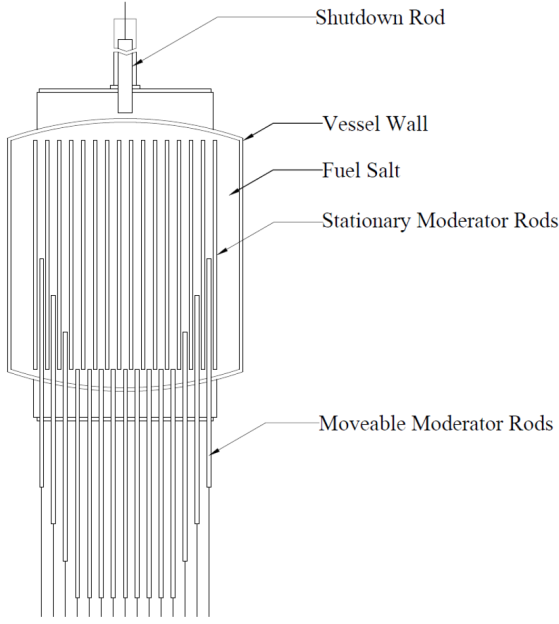
\includegraphics[width=0.65\textwidth]{tap_front_view.png}
  \caption{The \gls{TAP} \gls{MSR} schematic view showing movable moderator rod 
  bundles and shutdown rod (figure reproduced from Transatomic Power White Paper 
\cite{transatomic_power_corporation_technical_2016}).}
  \label{fig:tap-main-view}
\end{figure}

The \gls{TAP} \gls{MSR} primary loop contains the reactor core volume (including 
the zirconium hydride moderator rods with silicone carbide cladding), pumps, and 
primary heat exchanger. Pumps circulate the LiF-(Act)F$_4$ 
fuel salt through the primary loop. The pumps, vessels, tanks, and piping are 
made of a nickel-based alloy (similar to Hastelloy-N\footnote{ Hastelloy-N is 
very common in reactors now but have been studied and developed at \gls{ORNL} in 
a program that started in 1950s.}), which is highly resistant to corrosion in 
various molten 
salt environments. 
Inside the reactor vessel, in close proximity to the zirconium hydride moderator 
rods, the fuel salt is in a critical configuration and generates heat. 
Table~\ref{tab:tap_tab} contains details of the \gls{TAP} system 
design which are taken from technical white paper \cite{transatomic_power_corporation_technical_2016} 
and a neutronics overview
 \cite{transatomic_power_corporation_neutronics_2016} as well as \gls{ORNL} 
analysis of the \gls{TAP} 
design \cite{betzler_two-dimensional_2016, betzler_assessment_2017}. 
%%%%%%%%%%%%%%%%%%%%%%%%%%%%%%%%%%%%%%%%
\begin{table}[h!]
        \caption{Summary of principal data for the \gls{TAP} \gls{MSR} 
        (reproduced from \cite{transatomic_power_corporation_technical_2016, betzler_assessment_2017}). }
        \begin{tabularx}{\textwidth}{ s  s}
        \hline
         Thermal power				           		& 1250 MW$_{th}  $       \\ 
         Electric power		                		& 520 MW$_e  $ 			 \\ 
         Gross thermal efficiency        			& 44\%     				 \\  
         Outlet temperature							& 620$^{\circ}$C         \\ 
		 Fuel salt components                   & LiF-UF$_4$				 \\  
 		 Fuel salt composition                  & 72.5-27.5 mole\%			 \\  
         Uranium enrichment                     & 5\% $^{235}$U          	 \\
         Moderator                              & Zirconium Hydride (ZrH$_{1.66}$) rods (with silicon carbide cladding) \\
	     Neutron spectrum						& thermal/epithermal                 \\
         \hline
        \end{tabularx}
        \label{tab:tap_tab}
\end{table}
%%%%%%%%%%%%%%%%%%%%%%%%%%%%%%%%%%%%%%%%%%%%%%%%
\subsection{TAP core design}
In the \gls{TAP} core (figure~\ref{fig:tap-core-view}), fuel salt flows around 
moderator assemblies consisting 
of lattices of 
zirconium hydride rods clad in a corrosion-resistant silicone carbide 
(figure~\ref{fig:tap-main-view}). The \gls{TAP} reactor pressure vessel is a 
cylinder with an inner radius 150 cm, height 350 cm, and wall thickness 5 cm made 
of a nickel-based alloy. The moderator-to-fuel ratio, or salt volume fraction 
(SVF), in the core can be varied during operation to 
shift the spectrum from intermediate to thermal energies (from \gls{BOL} to 
\gls{EOL}, respectively) to maximize fuel burnup. In practice, SVF can be 
varied by inserting fixed-sized moderator rods via the bottom of the reactor 
vessel (for safety considerations), similarly to moving the control rods in 
a \gls{BWR}, as shown in Figure~\ref{fig:tap-main-view}. For the \gls{TAP} 
reactor, \gls{EOL} occurs when the maximum number of moderator rods are 
inserted into the core and further injection of fresh fuel salt does not 
change a criticality. Unmoderated salt is flowing in the annulus 
between the core and the vessel wall provides for a potential reduction in 
fast neutron flux at the vessel structural material  \cite{transatomic_power_corporation_neutronics_2016}.
\begin{figure}[t] % replace 't' with 'b' to 
		  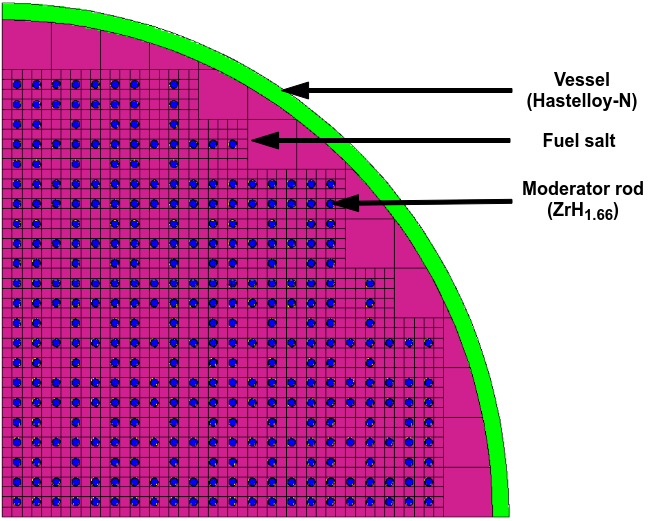
\includegraphics[width=\textwidth]{tap_core_ornl.png}
	  	\vspace{-0.35in}
  \caption{The \gls{TAP} \gls{MSR} schematic core view showing moderator rods 
  (figure reproduced from ORNL/TM-2017/475  
\cite{betzler_assessment_2017}).}
  \label{fig:tap-core-view}
\end{figure}

\subsection{TAP reprocessing system structure and simulation approach}
The \gls{TAP} nuclear island contains \gls{FP} removal system. Gaseous 
\glspl{FP} are continuously removed using an off-gas system while liquid 
and solid \glspl{FP} are extracted via a chemical processing system. As 
these byproducts are gradually removed, a small quantity 
of fresh fuel salt is regularly added to the primary loop. This process conserves a 
constant fuel salt mass and keeps the reactor critical. In contrast with the \gls{MSBR} 
reprocessing system, the \gls{TAP} does not need a protactinium separation and isolation 
system because it operates in a uranium-based single-stage fuel cycle. The authors of 
the \gls{TAP} concept suggested three distinct fission product removal methods 
\cite{transatomic_power_corporation_neutronics_2016}:
\paragraph{Off-Gas System:} Removes gaseous fission products such as krypton 
and xenon, 
which are then compressed and stored temporarily until they have decayed to the 
background 
radiation level. Trace amounts of tritium are also removed and bottled in a liquid 
form via the same process. Also, the off-gas system also directly 
removes a small fraction of the noble metals.
\paragraph{Metal Plate-Out/Filtration:} Removes noble and semi-noble metal 
solid fission 
products as they plate out onto a nickel mesh filter located in a side stream in the 
primary loop.
\paragraph{Liquid Metal Extraction:} Lanthanides and other non-noble 
metals stay dissolved in the fuel salt. They generally have a lower capture cross 
section and thus absorb fewer neutrons than $^{135}$Xe but their extraction is essential 
to ensuring normal operation. In the \gls{TAP} reactor, lanthanides removal is
accomplished via 
a liquid-metal/molten salt extraction process similar to that developed for \gls{MSBR} 
by \gls{ORNL} \cite{robertson_conceptual_1971}. The process 
converts the dissolved lanthanides into a well-understood oxide waste form, similar to 
that of \gls{LWR} \gls{SNF}. This oxide waste comes out of the \gls{TAP} reprocessing 
plant in ceramic granules and can be sintered into another convenient form for storage.

Figure~\ref{fig:tap-reproc} shows a principal design of the \gls{TAP} primary 
loop including an off-gas system, nickel mesh filter, and lanthanide chemical 
extraction facility. Similarly to \gls{MSBR}, an off-gas system is 
also based on a simple process of helium sparging through fuel salt 
with consequent gas bubbles removed before returning the 
fuel salt back to the core. Nevertheless, one important difference must be noted: the
\gls{MSBR} gas separation system suggested helium injection and subsequent 
transport of the voids throughout the primary loop, including the core 
for at least 10 full loops \cite{robertson_conceptual_1971}. It is a 
significant concern to safe, stable 
operation because the increase of void fraction in the fuel salt when it enters back 
to the core 
would cause unpredictable reactivity change. This drawback can be overcome by 
using an effective gas separator for stripping helium/xenon bubbles before 
returning the salt back to a primary loop (Figure~\ref{fig:tap-reproc}, blue 
block). 
\begin{figure}[htp!] % replace 't' with 'b' to 
  \centering
		  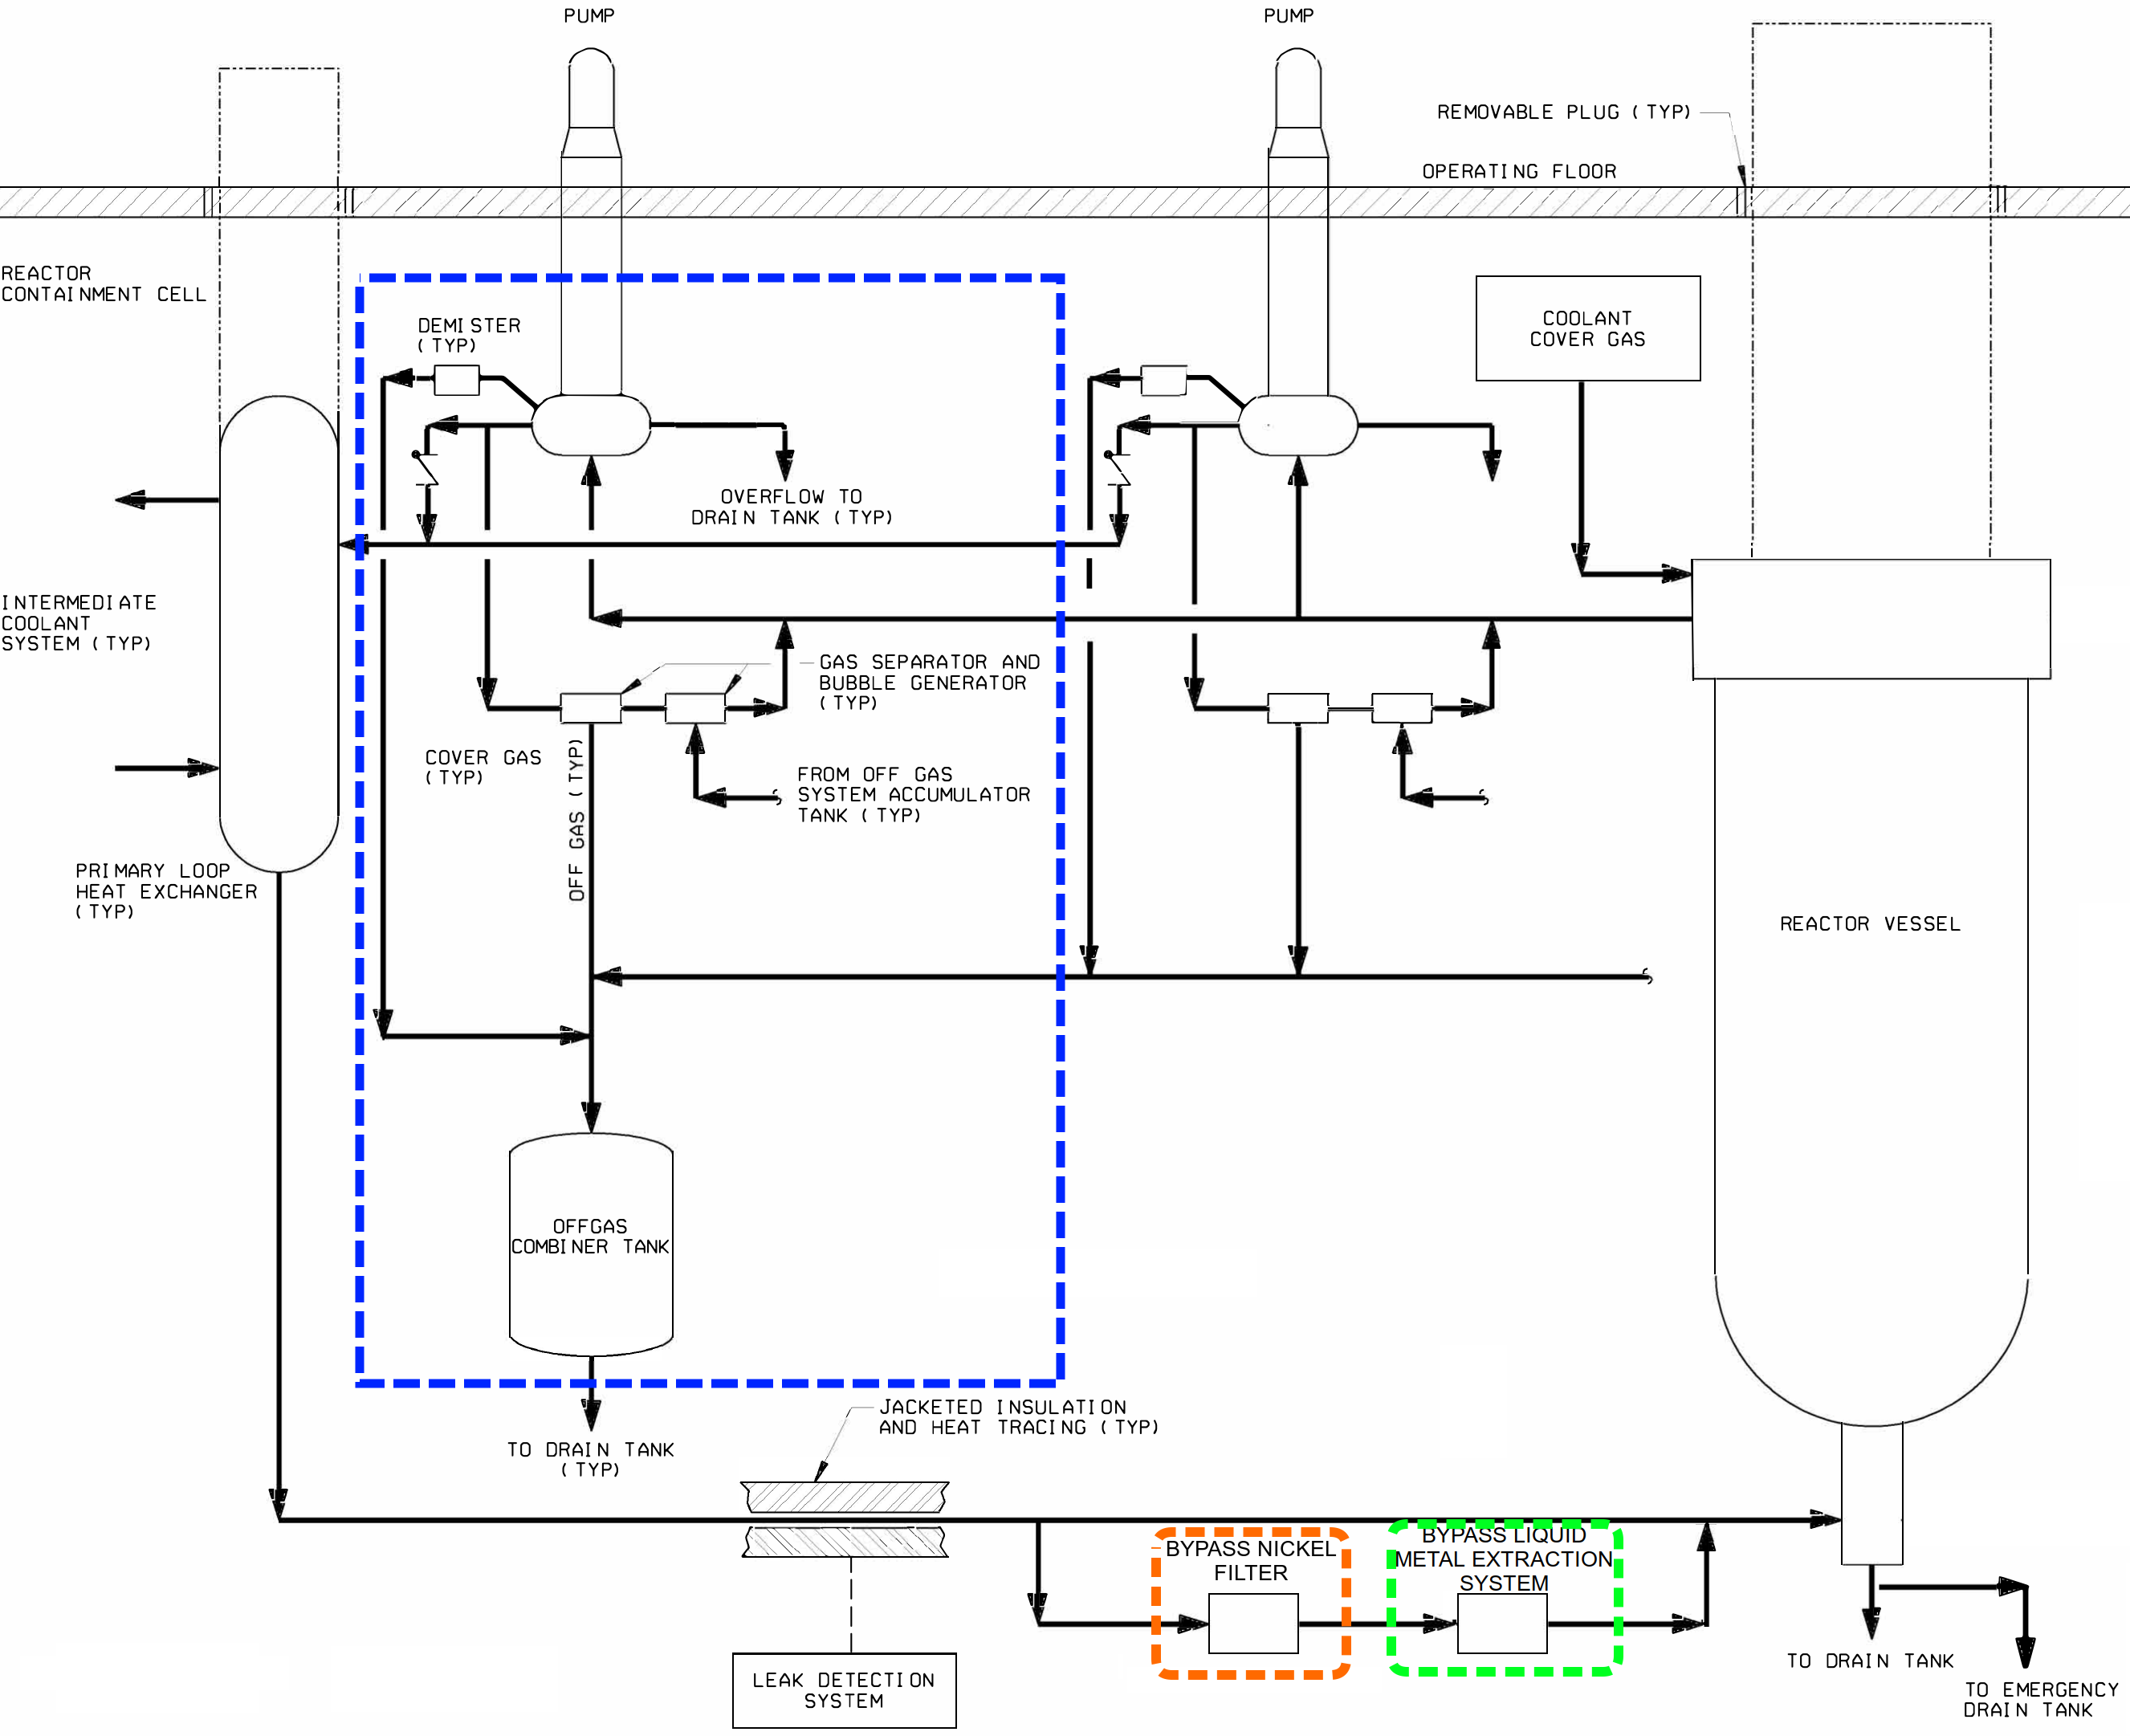
\includegraphics[width=\textwidth]{tap_primary_loop.png}
  \caption{Simplified \gls{TAP} primary loop design including off-gas system (blue), 
  nickel filter (orange) and liquid metal extraction system (green) (reproduced from \cite{transatomic_power_transatomic_2019}).}
  \label{fig:tap-reproc}
\end{figure}

Noble and semi-noble metal solid fission products tend to plate out onto metal 
surfaces including piping, heat exchanger tubes, reactor vessel inner surface, etc. 
Previous research by \gls{ORNL} \cite{robertson_conceptual_1971} reported that 
about 50\% of noble and semi-noble metals would plate out inside \gls{MSBR} 
systems without any special treatment. To improve the extraction efficiency of 
these fission products, the \gls{TAP} concept suggested employing a 
nickel mesh filter located 
in a bypass stream in the primary loop (Figure~\ref{fig:tap-reproc}, orange block). 
The main idea of this filter is to create a maze with large metal (nickel) 
surface area. The fuel salt flowing throughout the filter and noble 
metals plate-out on the filter internal surface. 

This Liquid Metal Extraction process for the \gls{TAP} concept has been adopted from 
the \gls{MSBR}. The \gls{MSRE} demonstrated a liquid-liquid extraction process 
for removing rare earths and lanthanides from fuel salt and estimated efficiency 
of this process.

The \gls{TAP} project reported detailed list of elements for removal and removal 
efficiencies (Table~\ref{tab:reprocessing_list}). We used data from \gls{TAP} 
neutronics whitepaper\cite{transatomic_power_corporation_neutronics_2016} for 
SaltProc v2.0+  demonstration case without any modifications.
%%%%%%%%%%%%%%%%%%%%%%%%%%%%%%%%%%%%%%%%
\begin{table}[ht!]
        \centering
        \caption{The effective cycle times for fission products removal (reproduced from \cite{betzler_implementation_2017} and \cite{transatomic_power_corporation_neutronics_2016}).}
        \begin{tabular}{p{0.2\textwidth} p{0.42\textwidth} p{0.12\textwidth} p{0.16\textwidth}}
        \hline 
        %\begin{tabularx}{\linewidth}{l X} \toprule 
        Processing group & \qquad\qquad\qquad Nuclides & Removal Rate (s$^{-1}$) & Cycle time (at full power) \\ [5pt] \hline 
 \multicolumn{3}{c}{\textit{Elements removed in \gls{MSBR} concept and adopted for the \gls{TAP}} \cite{robertson_conceptual_1971}} \\
        Volatile gases & Xe, Kr								  & 5.00E-2 & 20 sec \\ [5pt]
        Noble metals & Se, Nb, Mo, Tc, Ru, Rh, Pd, Ag, Sb, Te & 5.00E-2 & 20 sec \\ [5pt]
        Seminoble metals & Zr, Cd, In, Sn	  				  & 5.79E-8 & 200 days \\ [5pt]
        Volatile fluorides & Br, I 							  & 1.93E-7 & 60 days \\ [5pt]
        Rare earths & Y, La, Ce, Pr, Nd, Pm, Sm, Gd           & 2.31E-7 & 50 days \\ [5pt]
        \qquad & Eu & 2.32E-8 & 500 days \\ [5pt]
        Discard & Rb, Sr, Cs, Ba & 3.37E-9 & 3435 days \\ [5pt] 
        \hline
 
 \multicolumn{3}{c}{\textit{Additional elements removed} \cite{transatomic_power_corporation_neutronics_2016, betzler_implementation_2017}  } \\
        Volatile gases & H								  	& 5.00E-2 & 20 sec    \\ [5pt]
        Noble metals & Ti, V, Cr, Cu						& 3.37E-9 & 3435 days \\ [5pt]
        Seminoble metals & Mn, Fe, Co, Ni, Zn, Ga, Ge, As   & 3.37E-9 & 3435 days \\ [5pt]
        Rare earths & Sc									& 3.37E-9 & 3435 days \\ [5pt]
        Discard & Ca										& 3.37E-9 & 3435 days \\ [5pt] 
        \hline
        \end{tabular}
        \label{tab:reprocessing_list}
          \vspace{-0.9em}
\end{table}

We simulated \gls{TAP} \gls{MSR} depletion in SaltProc v2.0+ using  
reprocessing cycle times from 
this section (Table~\ref{tab:reprocessing_list}), an online reprocessing 
system design details, and full-core reactor Serpent model 
(section~\ref{sec:tap_model})
 to capture the dynamics of fuel composition evolution during reactor operation.

\section{The SaltProc modeling and simulation code} \label{sec:tool}
The first version of the SaltProc Python tool for calculating \gls{MSR} fuel 
composition evolution taking into account an online reprocessing system 
was developed in 2018 as a part of M.S. thesis \cite{rykhlevskii_advanced_2018,
rykhlevskii_arfc/saltproc_2018}. The tool was designed to 
expand Serpent 2 depletion capabilities for modeling liquid-fueled \gls{MSR} 
with online fuel reprocessing system. SaltProc v1 uses HDF5 
\cite{the_hdf_group_hierarchical_1997} to store 
data and uses the PyNE Nuclear Engineering Toolkit \cite{scopatz_pyne_2012}
for Serpent 2 output file parsing and nuclide naming. SaltProc v1 is an 
open-source Python package that uses a batch-wise approach to simulate 
continuous feeds and removals in \glspl{MSR}. 

SaltProc v1 only allows 100\% separation efficiency for 
either specific elements or groups of elements (e.g., Processing Groups as described in 
Table~\ref{tab:reprocessing_list}) at the end of the specific cycle time. 
This simplification neglects the reality that the salt spends appreciable time 
out of the core, in the primary loop pipes and the heat exchanger. This approach 
works well for fast-removing elements (gases, noble metals) 
which should be removed each depletion step. Unfortunately, 
for the elements with longer cycle times (i.e. rare earths should be removed 
every 50 days) this simplified approach leads to oscillatory behavior of all
major parameters \cite{rykhlevskii_modeling_2019}. 

Capabilities of the developed tool, working with the Monte Carlo software 
Serpent 2, were demonstrated using the full-core MSBR design for a 
simplified case with ideal removal efficiency (100\% of mass for target 
elements removed) \cite{rykhlevskii_modeling_2019}. The preliminary version of 
SaltProc architecture and principal structure was not designed for 
flexible implementation of sophisticated online reprocessing systems 
including realistic physics/chemistry-based extraction efficiencies. 

We completely re-factored SaltProc v1 using \gls{OOP} to create a 
comprehensive generic tool to realistically model any \gls{MSR} 
reprocessing plant while taking into account non-ideal or variable extraction 
efficiencies, and mass balance between the core and processing plant.

\subsection{SaltProc v2.0+ architecture}
The SaltProc v2.0+ Python toolkit coupled directly with Serpent 2 input 
and output files, to allow the reprocessing system couples to depletion calculation. 
Existing PyNE interfaces are employed for Serpent output parsing as 
well as newly developed interfaces for input and output handling. 
Python 3 \gls{OOP} standard features is used to create a flexible, 
user-friendly tool with great potential for further improvement and 
collaboration. 
Figure~\ref{fig:saltproc_class} shows the SaltProc v2.0+ class structure 
which includes 4 main classes:
\begin{figure}[ht!] % replace 't' with 'b' to \centering
  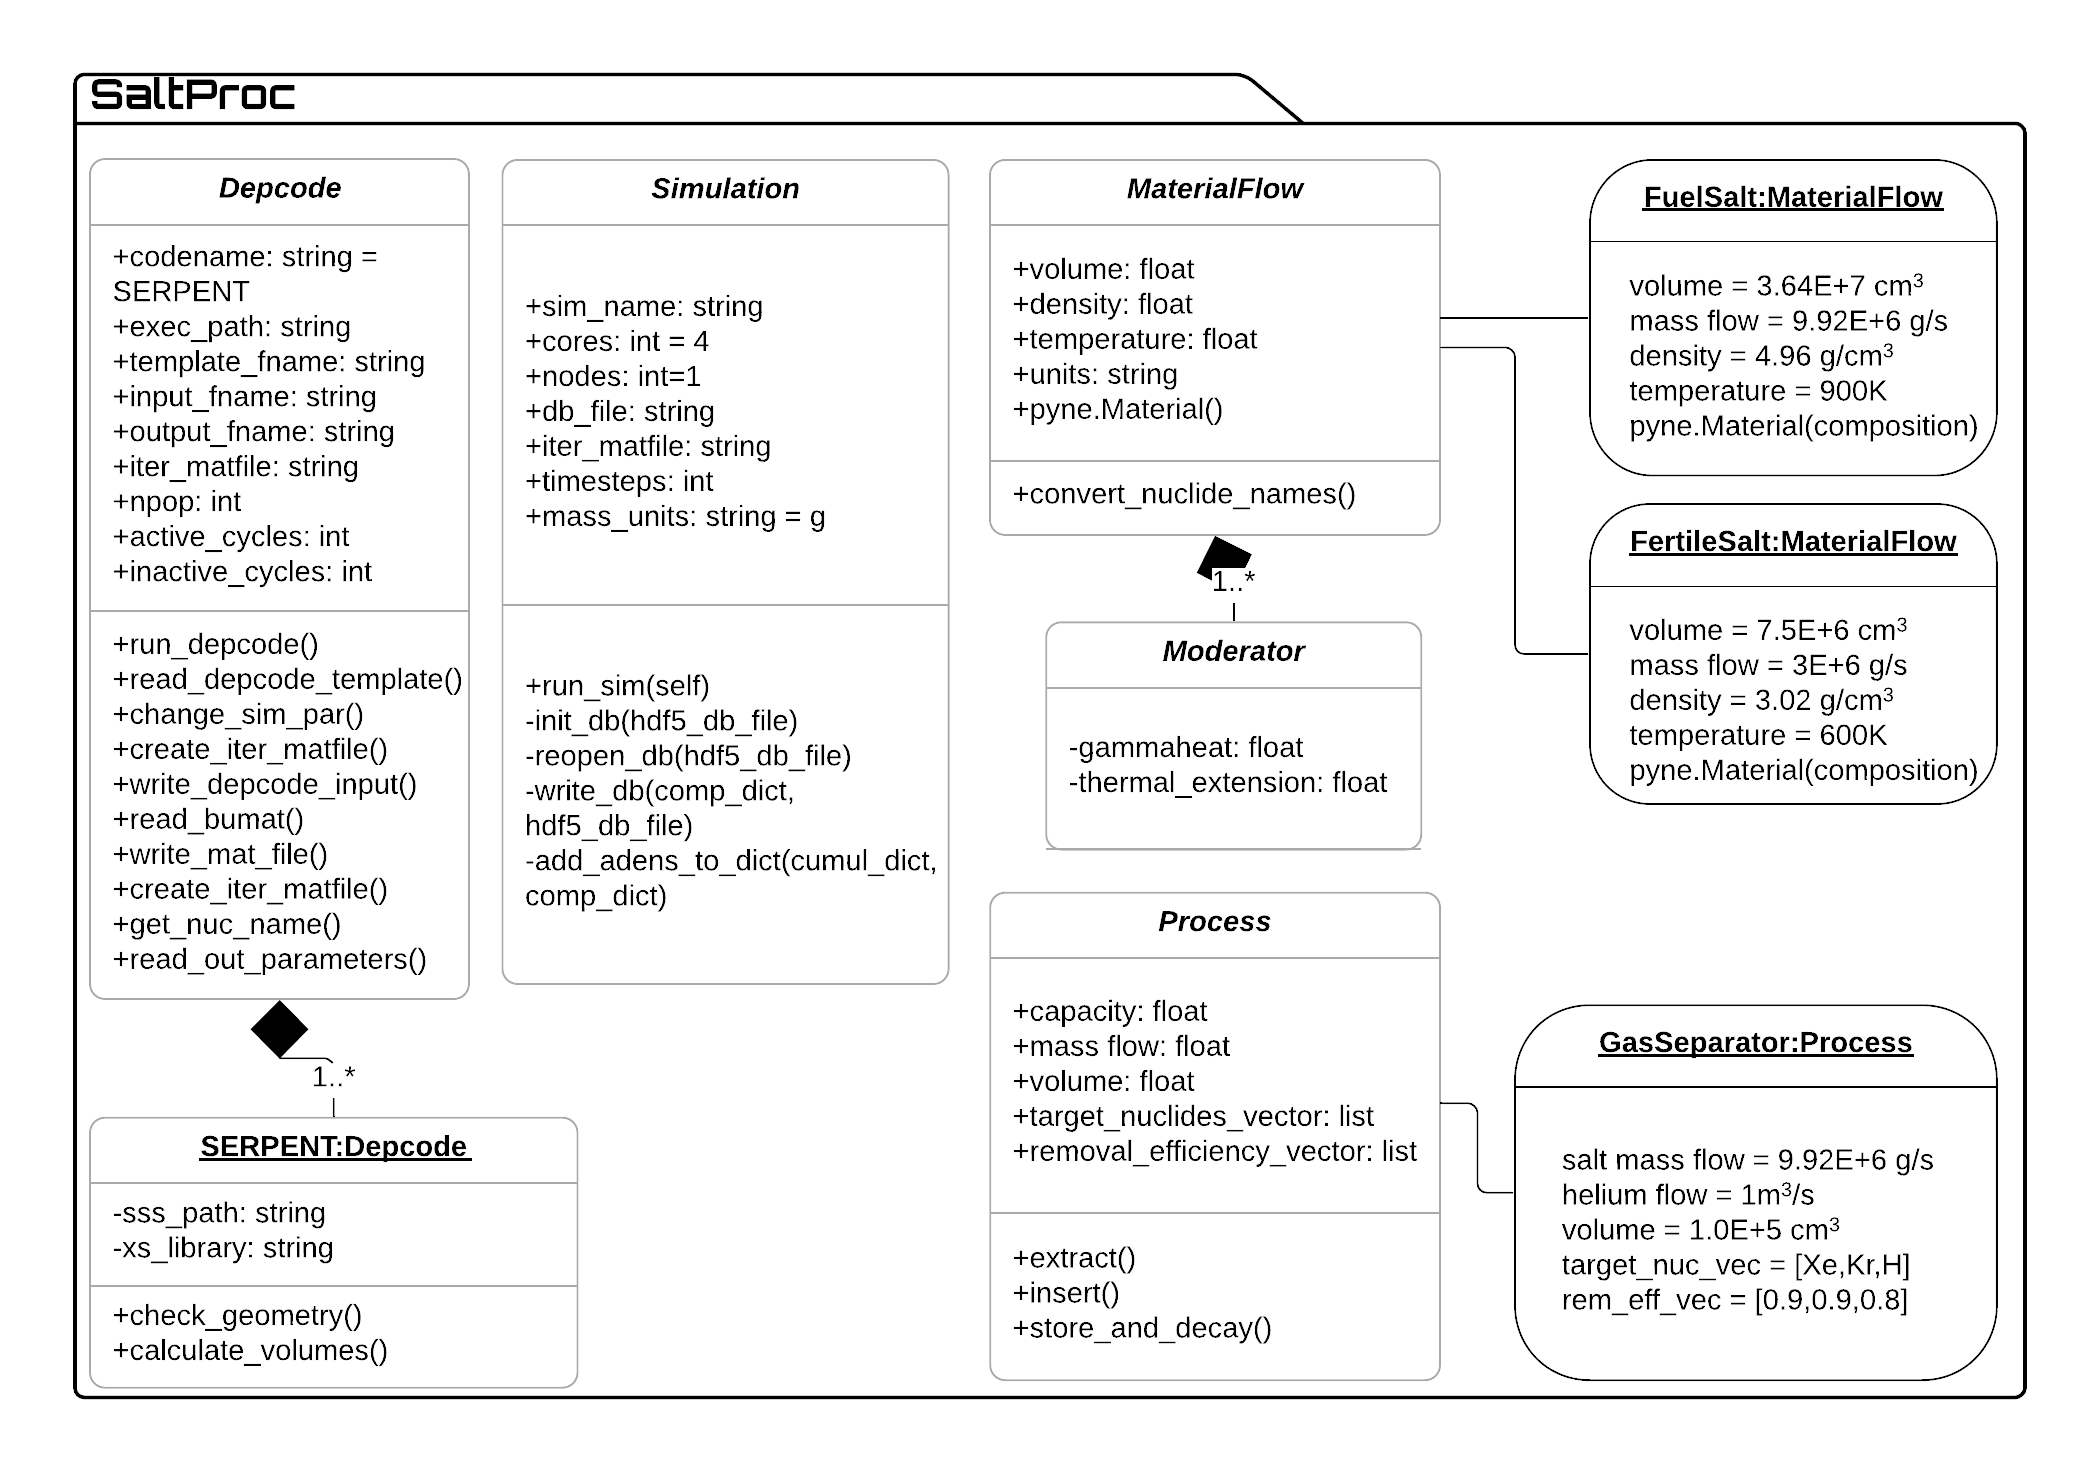
\includegraphics[width=1.07\textwidth]{saltproc_class_diagram.png}
  	  	\vspace{-0.35in}
  \caption{SaltProc v2.0+ python package class diagram in UML notation 
  and examples of object instances.}
  \label{fig:saltproc_class}
\end{figure}
	\paragraph{Depcode.}Contains attributes and methods for 
	reading the user's input file for the depletion software, initial 
	material (e.g., fuel and/or fertile salt) composition, principal 
	parameters for 
	burnup simulation (e.g., neutron population and number of cycles for Monte 
	Carlo neutron transport), and running the depletion code.
	\paragraph{Simulation.} Runs Serpent depletion step, 
	creates and writes HDF5 database, tracks time and converts 
	isotopic composition vector nuclide names from Serpent to human-readable format.
	\paragraph{MaterialFlow.}Each \textit{MaterialFlow} object 
	represents the material flowing between \textit{Process} objects. 
	All instances of this class contain an isotopic composition vector 
	(PyNE Material object initialized from Serpent output file 
	\textbf{dep.m}), mass flow rate, 
	temperature, density, volume, and void fraction. Existing PyNE Material 
	capabilities allows to easily convert the units of isotopic 
	composition vector (e.g., from atomic density provided by Serpent to 
	a mass fraction or absolute mass in desired units), decay material 
	(i.e. model the \gls{MSBR} protactinium decay tank), calculate 
	decay heat, activity, and dose. The main idea of the \textit{MaterialFlow} 
	object is to pass detailed information about the salt starting at the 
	\gls{MSR} vessel outlet throughout reprocessing components 
	(\textit{Processes}), which modify the \textit{MaterialFlow} 
	object before depleting the material in the next Serpent burnup step.
	\paragraph{Process.}Each \textit{Process} object represents a 
	realistic fuel processing step characterized by its throughput rate, 
	volumetric capacity, extraction efficiency for each target element (can be 
	a function of many parameters), waste streams, and other parameters specific 
	to the particular process. Feed	\textit{Process} injects fresh fuel salt 
	\textit{MaterialFlow} directly into the reactor core (e.g., adding fissile 
	material with a specific mass flow rate to \textit{MaterialFlow} after 
	performing all removals).

The proposed class structure provides outstanding flexibility in simulating 
various \gls{MSR} fuel processing system designs. A library of various 
\textit{MaterialFlow} (e.g., 
fuel salt flow, fertile salt flow, refueling salt flow) and \textit{Process} 
(e.g., helium sparging facility, gas separator, lanthanide removal component) 
objects will be created to allow a user to quickly create a model 
of a desired reprocessing scheme. At runtime, the user will connect 
\textit{Process} objects in series or parallel with \textit{MaterialFlow} 
objects to form a comprehensive reprocessing system. The user will also be 
able to create custom objects with desired attributes and methods, and 
contribute back to the code package using GitHub (https://github.com/ arfc/saltproc).	

\subsection{SaltProc v2.0+ flowchart}
Figure~\ref{fig:saltproc_flow} illustrates the online reprocessing simulation 
algorithm coupling SaltProc v2.0+ and Serpent. To perform a depletion step, 
SaltProc v2.0+ reads a user-defined Serpent template file. This file contains input 
 parameters such as geometry, material, isotopic composition, neutron 
population, criticality cycles, total heating power, and boundary conditions. 
SaltProc v2.0+ fills in the template file and runs Serpent single-step depletion. 
After the depletion calculation, SaltProc v2.0+ reads the depleted fuel composition 
file into \textit{MaterialFlow} object (\textit{core\textunderscore outlet} in 
figure~\ref{fig:saltproc_flow}). This object contains an isotopic composition 
vector, total volume of material, total mass, mass flow rate, density, temperature, 
void fraction, etc. For the simplest reprocessing case, when all fuel 
processing components are located in-line 
(100\% of total material flow goes through 
a chain of separation components), the \textit{core\textunderscore outlet} object is flowing 
sequentially between \textit{Processes} and each \textit{Process} is 
removing a mass fraction of target elements with specified extraction 
efficiency. Afterward, the removed material mass is compensated by 
fresh fuel salt to maintain the salt inventory in a primary loop. 
Finally, resulting isotopic composition after reprocessing is stored in 
HDF5 database and dumped in a new composition file for the next 
Serpent depletion run. SaltProc v2.0+ also stores in database isotopic composition 
before reprocessing and waste stream from each fuel processing component. 
\begin{figure}[ht!] % replace 't' with 'b' to \centering
	\centering
  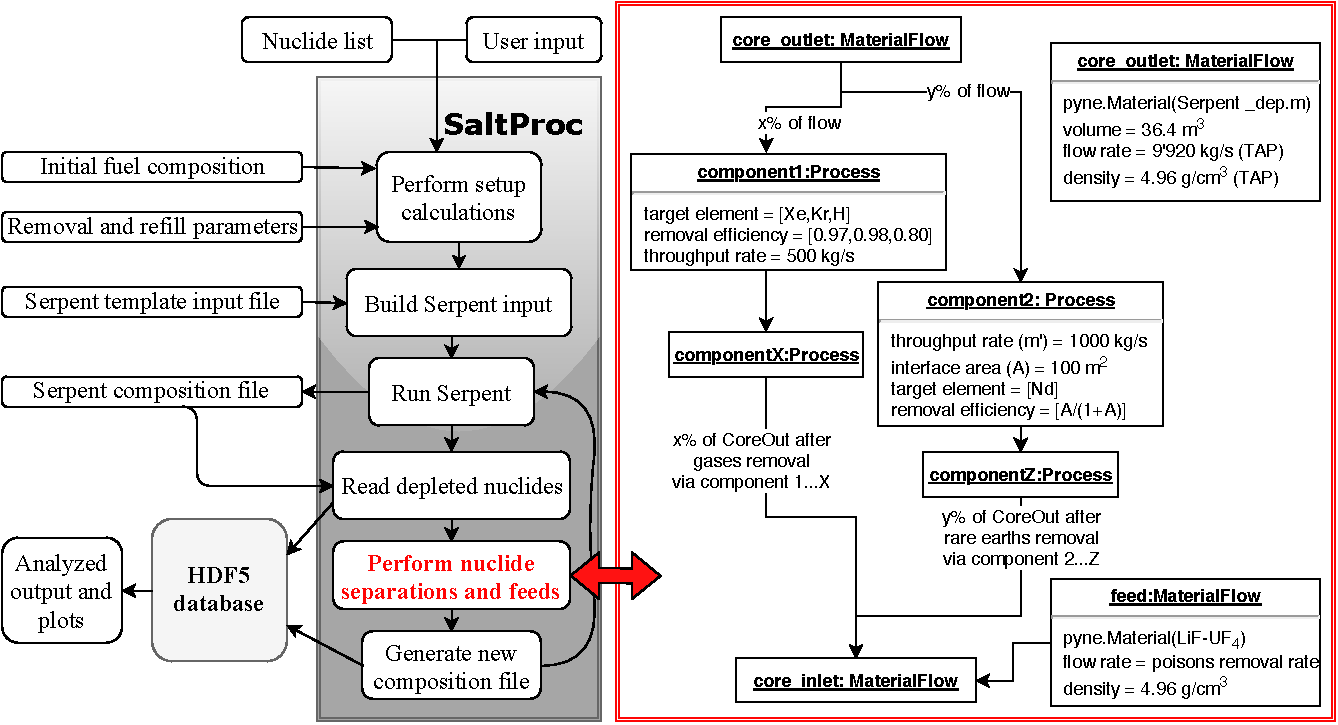
\includegraphics[width=1.03\textwidth]{saltproc_flowchart.pdf}
  	  	\vspace{-0.35in}
  \caption{SaltProc v2.0+ python package flow chart.}
  \label{fig:saltproc_flow}
\end{figure}

For a more general case with multiple concurrent extraction processes, a separate 
\textit{MaterialFlow} object is created for each branch with a user-defined 
mass flow rate (e.g. 90\% of total mass flow rate flows via left branch and 
10\% through a right branch). The total mass and isotopic composition vector 
for each \textit{MaterialFlow} object is calculated as a fraction of incoming 
\textit{core\textunderscore outlet} flow. Then each \textit{MaterialFlow} object is 
passed via a cascade of \textit{Processes} to separate selected chemical elements with 
specific efficiency. Finally, the left-hand-side branch \textit{MaterialFlow} object is
 merged with the right-hand-side and similarly to the previous case, fresh 
fuel salt feed compensate the loss of mass in separation facilities and keep 
fuel salt mass in a primary loop constant.

The class diagram (Figure~\ref{fig:saltproc_class}) allows to model 
the operation of a complex, multi-zone, 
multi-fluid \gls{MSR} and is sufficiently general to represent myriad reactor 
systems. The refactored version of SaltProc stores and edit the 
isotopic composition of the fuel stream, which makes it a flexible tool to 
model any geometry: an infinite medium, a unit cell, a multi-zone simplified 
assembly, or a full core. This flexibility allows the user to perform 
simulations of varying fidelity and computational intensity. SaltProc v2.0+ is an 
open-source tool (but a user needs Serpent installed to use SaltProc v2.0+), 
available on Github. It leverage unit and continuous tests  
crucial for sustainable development \cite{krekel_pytest_2004}. It will also 
have documentation generated through Sphinx, a documentation generator, for ease 
of use \cite{brandl_sphinx_2009}. In summary, the 
development approach of SaltProc v2.0+ is focused on producing a generic, flexible and 
expandable tool to give the Serpent 2 Monte Carlo code the ability to conduct 
advanced in-reactor fuel cycle analysis as well as simulate many 
online refueling and fuel reprocessing systems.

\section{SaltProc demonstration case}
The SaltProc v2.0+ modeling and simulation tool is demonstrated
for \gls{TAP} \gls{MSR} with static core geometry, \gls{LEU} 5\% 
startup composition 
\cite{transatomic_power_corporation_neutronics_2016} and following 
fueling scenarios: (1) no \glspl{FP} removal and feed (Serpent only);
(2) a 5\% \gls{LEU} online feed; (3) a 19.79\% 
\gls{LEU} online feed. 
The primary focus and the bulk of the analysis 
herein has been on the last fueling scenario using 
19.79\% \gls{LEU}. All calculations are run with 
Serpent version 2.1.31 and the JEFF-3.1.2 nuclear data library 
\cite{leppanen_serpent_2013, oecd/nea_data_bank_jeff-3.1.2_2014}.

\subsection{Serpent 2 full-core model} \label{sec:tap_model}
Advanced geometry surfaces and transformation capabilities of Serpent \cite{leppanen_serpent_2013} are employed 
to represent \gls{TAP} core. 
Figure~\ref{fig:tap-serpent-plan} shows the $XY$ section of whole-core
configuration at the expected reactor operational level when all
control rods are fully withdrawn. Figures~\ref{fig:tap-serpent-elev} and ~\ref{fig:tap-serpent-elev-zoom} show a 
longitudinal section of the reactor. This model contains the moderator rods with 
silicon carbide cladding, pressure vessel, and inlet and outlet plena 
(Table~\ref{tab:tap_model_param}). Fuel salt flows around rectangular 
moderator assemblies consisting of lattices of small-diameter zirconium hydride 
rods in a corrosion-resistant material. The \gls{SVF} in the core is parameter 
similar to wide-used moderator-to-fuel ratio and can be defined as:
\begin{align}
SVF &= \frac{V_F}{V_F+V_M} = \frac{1}{1+V_M/V_F}
	\intertext{where}
 	V_F &= \mbox{the fuel volume} \nonumber \\
 	V_M &= \mbox{the moderator volume} \nonumber \\
 	V_M/V_F &= \mbox{the moderator-to-fuel salt ratio} \nonumber
\end{align}
The \gls{SVF} for model herein is 0.907268 which means the modeled core is 
under-moderated and has intermediate spectrum.
\begin{figure}[htp!] % replace 't' with 'b' to 
  \centering
		  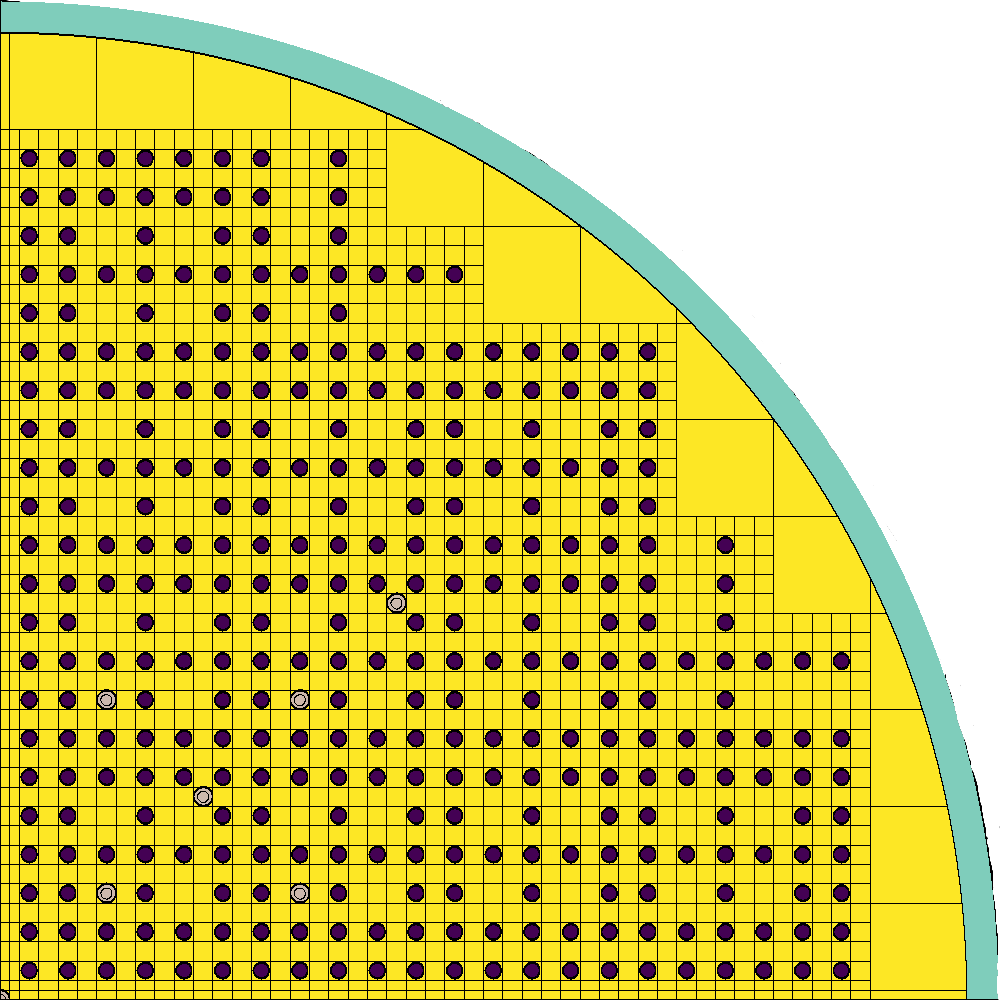
\includegraphics[width=\textwidth]{tap_plan_view.png}
  \caption{An $XY$ section of the \gls{TAP} model at horizontal midplane 
  with fully withdrawn control rods at \gls{BOL} (\gls{SVF}$=0.907268$). 
  The violet color represents zirconium 
hydride, and the yellow represents fuel salt. The blue color shows 
Hastelloy-N, a material used for the vessel wall, and the white color 
is the air.}
  \label{fig:tap-serpent-plan}
\end{figure}
\begin{figure}[htp!] % replace 't' with 'b' to 
  \centering
		  
\includegraphics[width=\textwidth]{tap_elev_view.png}
		 \vspace{-0.35in}
  \caption{An $XZ$ section of the \gls{TAP} model.}
  \label{fig:tap-serpent-elev}
\end{figure}
\begin{figure}[htp!] % replace 't' with 'b' to 
  \centering
		  \includegraphics[width=0.45\textwidth]{tap_elev_view_zoomed.png}
		 \vspace{-0.2in}
  \caption{Zoomed $XZ$ section of the top of the moderator rods and guide tubes for \gls{TAP} model. The orange color shows 70–30\% Gd$_2$O$_3$–Al$_2$O$_3$ ceramic 
absorbers used for control rods.}
  \label{fig:tap-serpent-elev-zoom}
\end{figure}

To represent reactivity control system the 
model has: (1) control rod guide tubes made of nickel-based alloy; (2) control rods represented as hollow 70-30\% Gd$_2$O$_3$-Al$_2$O$_3$ cylinders with a thin 
Hastelloy-N coating \cite{betzler_assessment_2017}; (3) air inside guide tubes and 
control rods. Control rods design has yielded a cluster of 25 rods that provide a total reactivity worth of 1121pcm\footnote{ 1 pcm = 10$^{-5}\Delta k_{eff}/k_{eff}$.}.

The control rod cluster is modeled using the
\textbf{TRANS} Serpent 2 feature which allows easily change the control rods 
position during simulation. 
Herein we assumed that all control rods are fully withdrawn from the core 
(figure~\ref{fig:tap-serpent-elev-zoom}) but for future investigation control 
rods position may vary. In this report, all figures of the core were 
generated using the built-in Serpent plotter.
%%%%%%%%%%%%%%%%%%%%%%%%%%%%%%%%%%%%%%%%%%%%%%%%%%
\begin{table}[h!]
        \caption{Geometric parameters for the full-core 3D model of 
        \gls{TAP} (reproduced from Betzler \emph{et al.} \cite{betzler_assessment_2017}). }
          \centering
        \begin{tabularx}{0.9\textwidth}{s s x p{0.15\textwidth}}
        \hline
\textbf{Component} & \textbf{Parameter} & Value      		& Unit		             \\ \hline
\multirow{4}{*}{\begin{tabular}[c]{@{}l@{}}Moderator\\ rod\end{tabular}} 
		 & Cladding thickness      	  			    & 0.10 & cm				 \\  
         & Radius 				      	  			& 1.15 & cm				 \\  
         & Length				      	  			& 3.0  & m				 \\  
         & Pitch				      	  			& 3.0  & cm  			 \\ \hline 

\multirow{2}{*}{\begin{tabular}[c]{@{}l@{}}Moderator\\ assembly\end{tabular}} 
         & Array				      	  			& 5 $\times$ 5 & rods$\times$rods \\  
         & Pitch				      	  			& 15.0 & cm    				 \\  \hline

\multirow{4}{*}{\begin{tabular}[c]{@{}l@{}}Core\end{tabular}}          
         & Assemblies  				   	  			& 268  & assemblies/core \\  
         & Inner radius			      	  			& 1.5  & m    				 \\  
         & Plenum height			   	  			& 25.0 & cm    				 \\  
         & Vessel wall thickness     	  			& 5.0 & cm    				 \\ \hline            
        \end{tabularx}
        \label{tab:tap_model_param}
\end{table}
%%%%%%%%%%%%%%%%%%%%%%%%%%%%%%%%%%%%%%%%%%%%%%%%
\subsection{Simulated fuel reprocessing system}
We thoroughly analyzed the original \gls{TAP} reprocessing system design 
(figure~\ref{fig:tap-reproc}) and neutron poisons removal rates 
(table~\ref{tab:reprocessing_list}) to determine suitable reprocessing 
scheme for SaltProc v2.0+ demonstration (figure~\ref{fig:demo-repro-scheme}).
\begin{figure}[htp!] % replace 't' with 'b' to 
  \centering
		  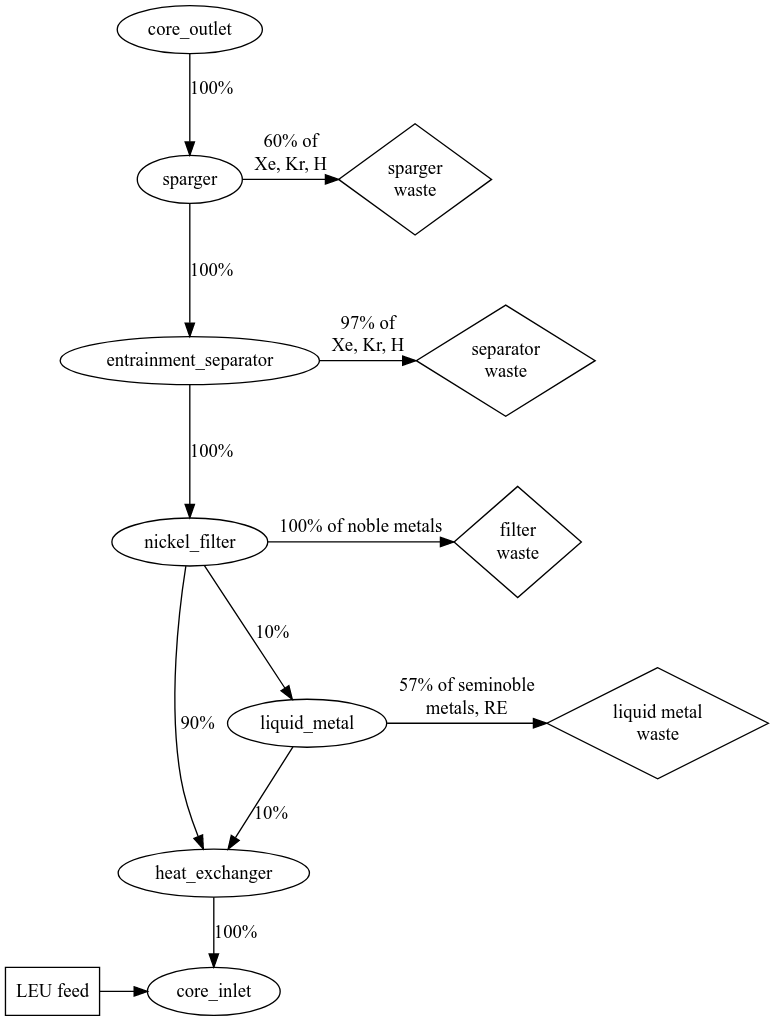
\includegraphics[width=0.93\textwidth]{demo_reprocessing_scheme.png}
  \caption{\gls{TAP} reprocessing scheme flowchart used for SaltProc v2.0+ 
  demonstration. Arrows represent material flows; percents - fraction of total 
  mass flow rate; ellipses - fuel reprocessing system 
  components; diamonds - waste streams; box shows refuel material flow.}
  \label{fig:demo-repro-scheme}
\end{figure}

The gas removal components (the sparger and entrainment separator) are located 
in-line because estimated full loop time for the fuel salt is about 
18 sec and approximately equal cycle time (table~\ref{tab:reprocessing_list}). 
To remove all volatile gases every 20 sec the fuel reprocessing system must 
operate with 100\% of the core throughout flow rate and exceptional efficiency. 
For the demonstration case herein to achieve required cycle time we assumed 
xenon, krypton, and hydrogen extraction efficiencies for the sparger and 
entrainment separator are equal 60\% and 97\%, respectively.

The nickel filter in the \gls{TAP} concept is designed to extract noble metals and 
volatile fluorides. Similarly to volatile gases, noble metals must be removed 
every 20 sec and, hence, the filter should also be able to operate in-line. 
The nickel filter removes a wide range of elements with various 
efficiencies. We calculated these efficiencies for SalProc v2.0+ input 
from removal rates reported in table~\ref{tab:reprocessing_list}.

Lanthanides and other non-noble metals generally have a lower capture cross-section 
and absorb fewer neutrons than gases and noble metals. These elements can be removed 
via a liquid-metal/molten salt extraction process with relatively low removal rates 
(cycle time > 50 days). This is accomplished using small fuel salt flow rate (10\% 
of the core throughout flow rate) via liquid-metal/molten salt component, 
where lanthanides are 
removed with specific extraction efficiency to match required cycle time 
(table~\ref{tab:reprocessing_list}). The rest 90\% of the flow is directed 
from the nickel filter to heat exchanger without performing any fuel salt treatment.

The removal rates vary among nuclides in this reactor concept, which dictate the 
necessary resolution of depletion calculations. If the depletion time intervals 
are very short, an enormous number of depletion steps are required to obtain 
the equilibrium composition. On the other hand, if the depletion calculation time 
interval is too long, the impact of short-lived fission products is not captured. To compromise, a 3-day time was selected based on Betzler \emph{et al.} timestep 
refinement study \cite{betzler_assessment_2017}. For longer, lifetime-long 
depletion simulations, 30-day timestep size will be applied.

\section{Results}
The SaltProc v2.0+ online reprocessing simulation package is demonstrated for 
analyzing \gls{TAP} \gls{MSR} neutronics and fuel cycle to find the equilibrium core composition and core depletion. The neutron population per cycle and the number 
of active/inactive cycles were chosen to obtain a balance between reasonable 
uncertainty for a transport problem (25 pcm for effective multiplication factor) 
and computational time. We accomplished it by setup neutron population 15'000, 
the number of active cycle 400, and the number of inactive cycle 200. 
The \gls{TAP} depletion was performed on 64 Blue Waters 
XE6 nodes (two AMD 6276 Interlagos CPU per node, 16 floating-point Bulldozer 
core units per node or 32 ``integer'' cores per node, nominal clock speed is 
2.45 GHz). The total computational time for calculating the equilibrium 
composition was approximately 9000 node-hours ($\approx$16 core-years).

\subsection{Effective multiplication factor}
Figures~\ref{fig:keff}, \ref{fig:keff-zoomed}, \ref{fig:keff-zoomed-2} demonstrate 
the effective 
multiplication factors  obtained using SaltProc v2.0+ and Serpent. We obtained 
the effective multiplication factors after removing fission products 
and adding feed material at the end of each depletion step (3 days for this 
work). The $k_{eff}$ fluctuates significantly as a result of the batch-wise 
nature of used online reprocessing strategy.
\begin{figure}[htp!] % replace 't' with 'b' to 
		  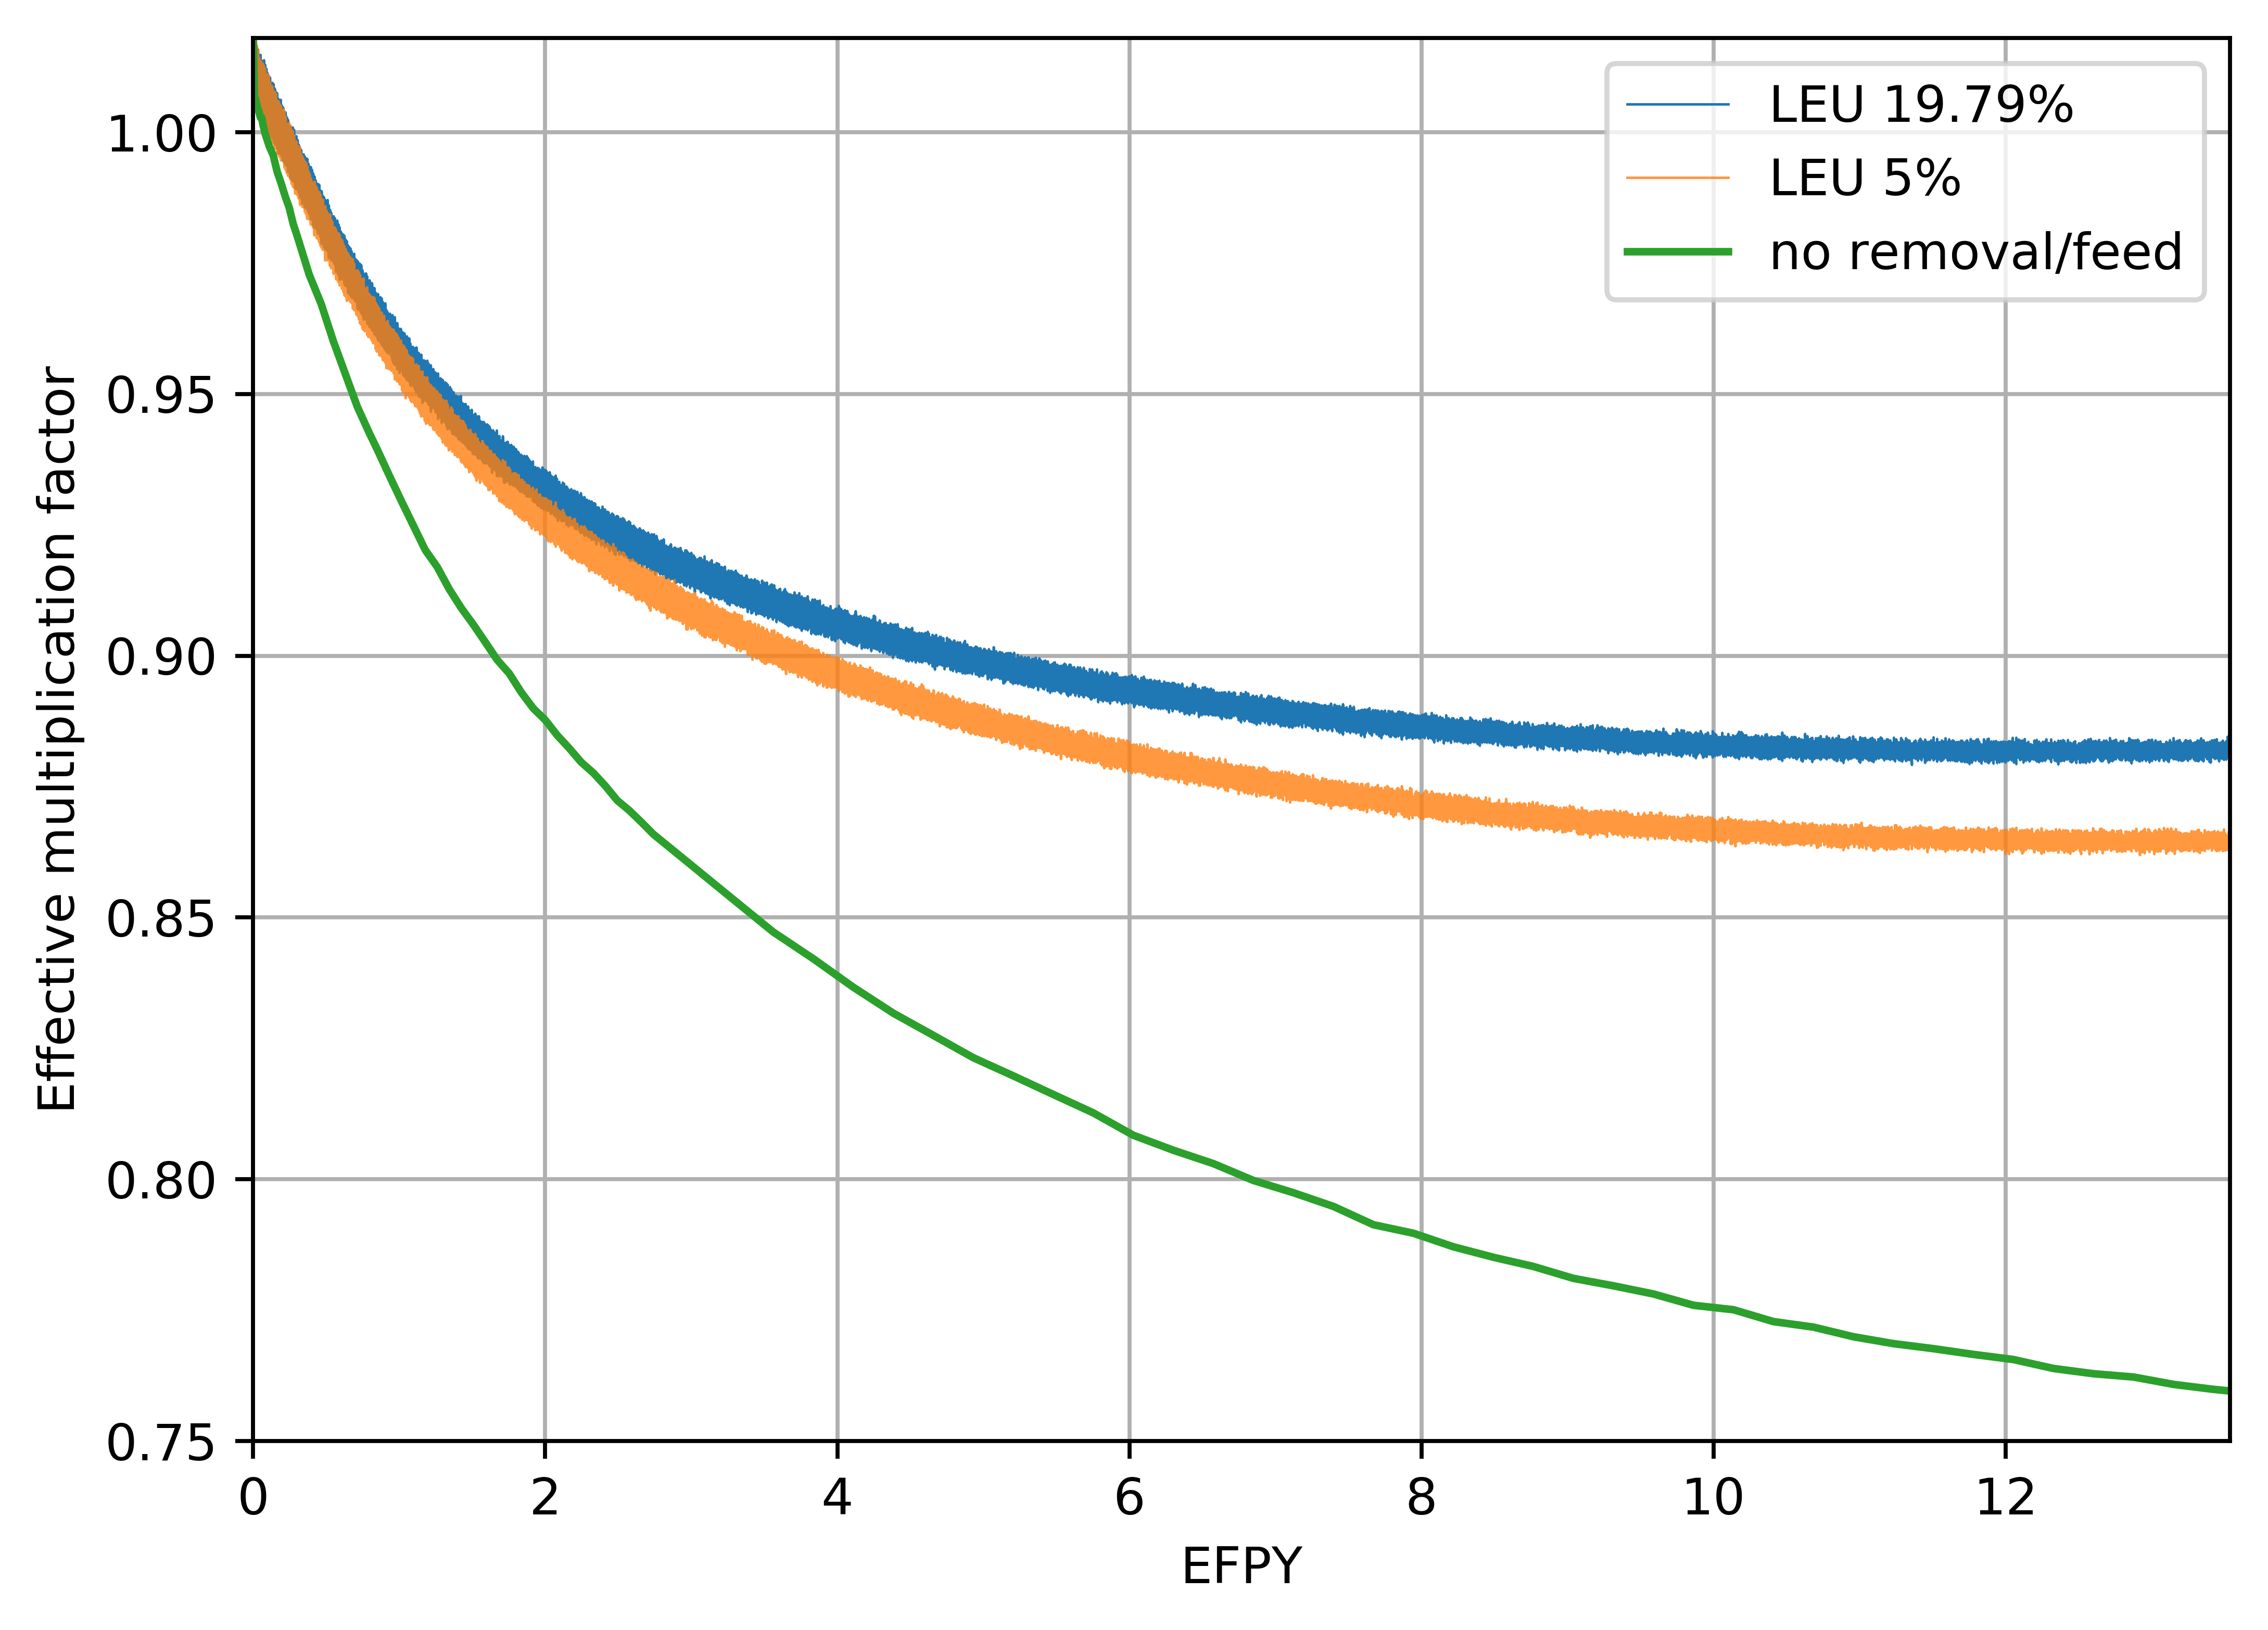
\includegraphics[width=1.05\textwidth]{keff_3.png}
	\vspace{-0.2in}
  \caption{Effective multiplication factor dynamics for full-core
   \gls{TAP} model for different fueling scenarios over a 13-year reactor operation. 
   Confidence interval $\pm\sigma=28pcm$ is shaded. Clearly, the reactor went 
   subcritical too fast and further investigation needed to overcome this issue. 
   Possible solutions are: (1) reduce neutron leakage from the core by 
   introducing thick graphite reflector and thermal insulation around 
   vessel to increase effective multiplication factor at the 
   \gls{BOL} to 1.035; (2) extract poisons with faster removal rate;
   (3) use another fissile material for the feed (i.e., \gls{TRU} elements from spent 
   \gls{LWR} fuel); (4) adjust \gls{SVF} on-the-fly by 
   moving moderator assemblies during operation 
   \cite{transatomic_power_corporation_technical_2016} or adding moderator rods 
   only at regular intervals during shutdown for reactor maintenance  \cite{betzler_fuel_2018}.}
  \label{fig:keff}
\end{figure}
\begin{figure}[htp!] % replace 't' with 'b' to 
  \centering
		  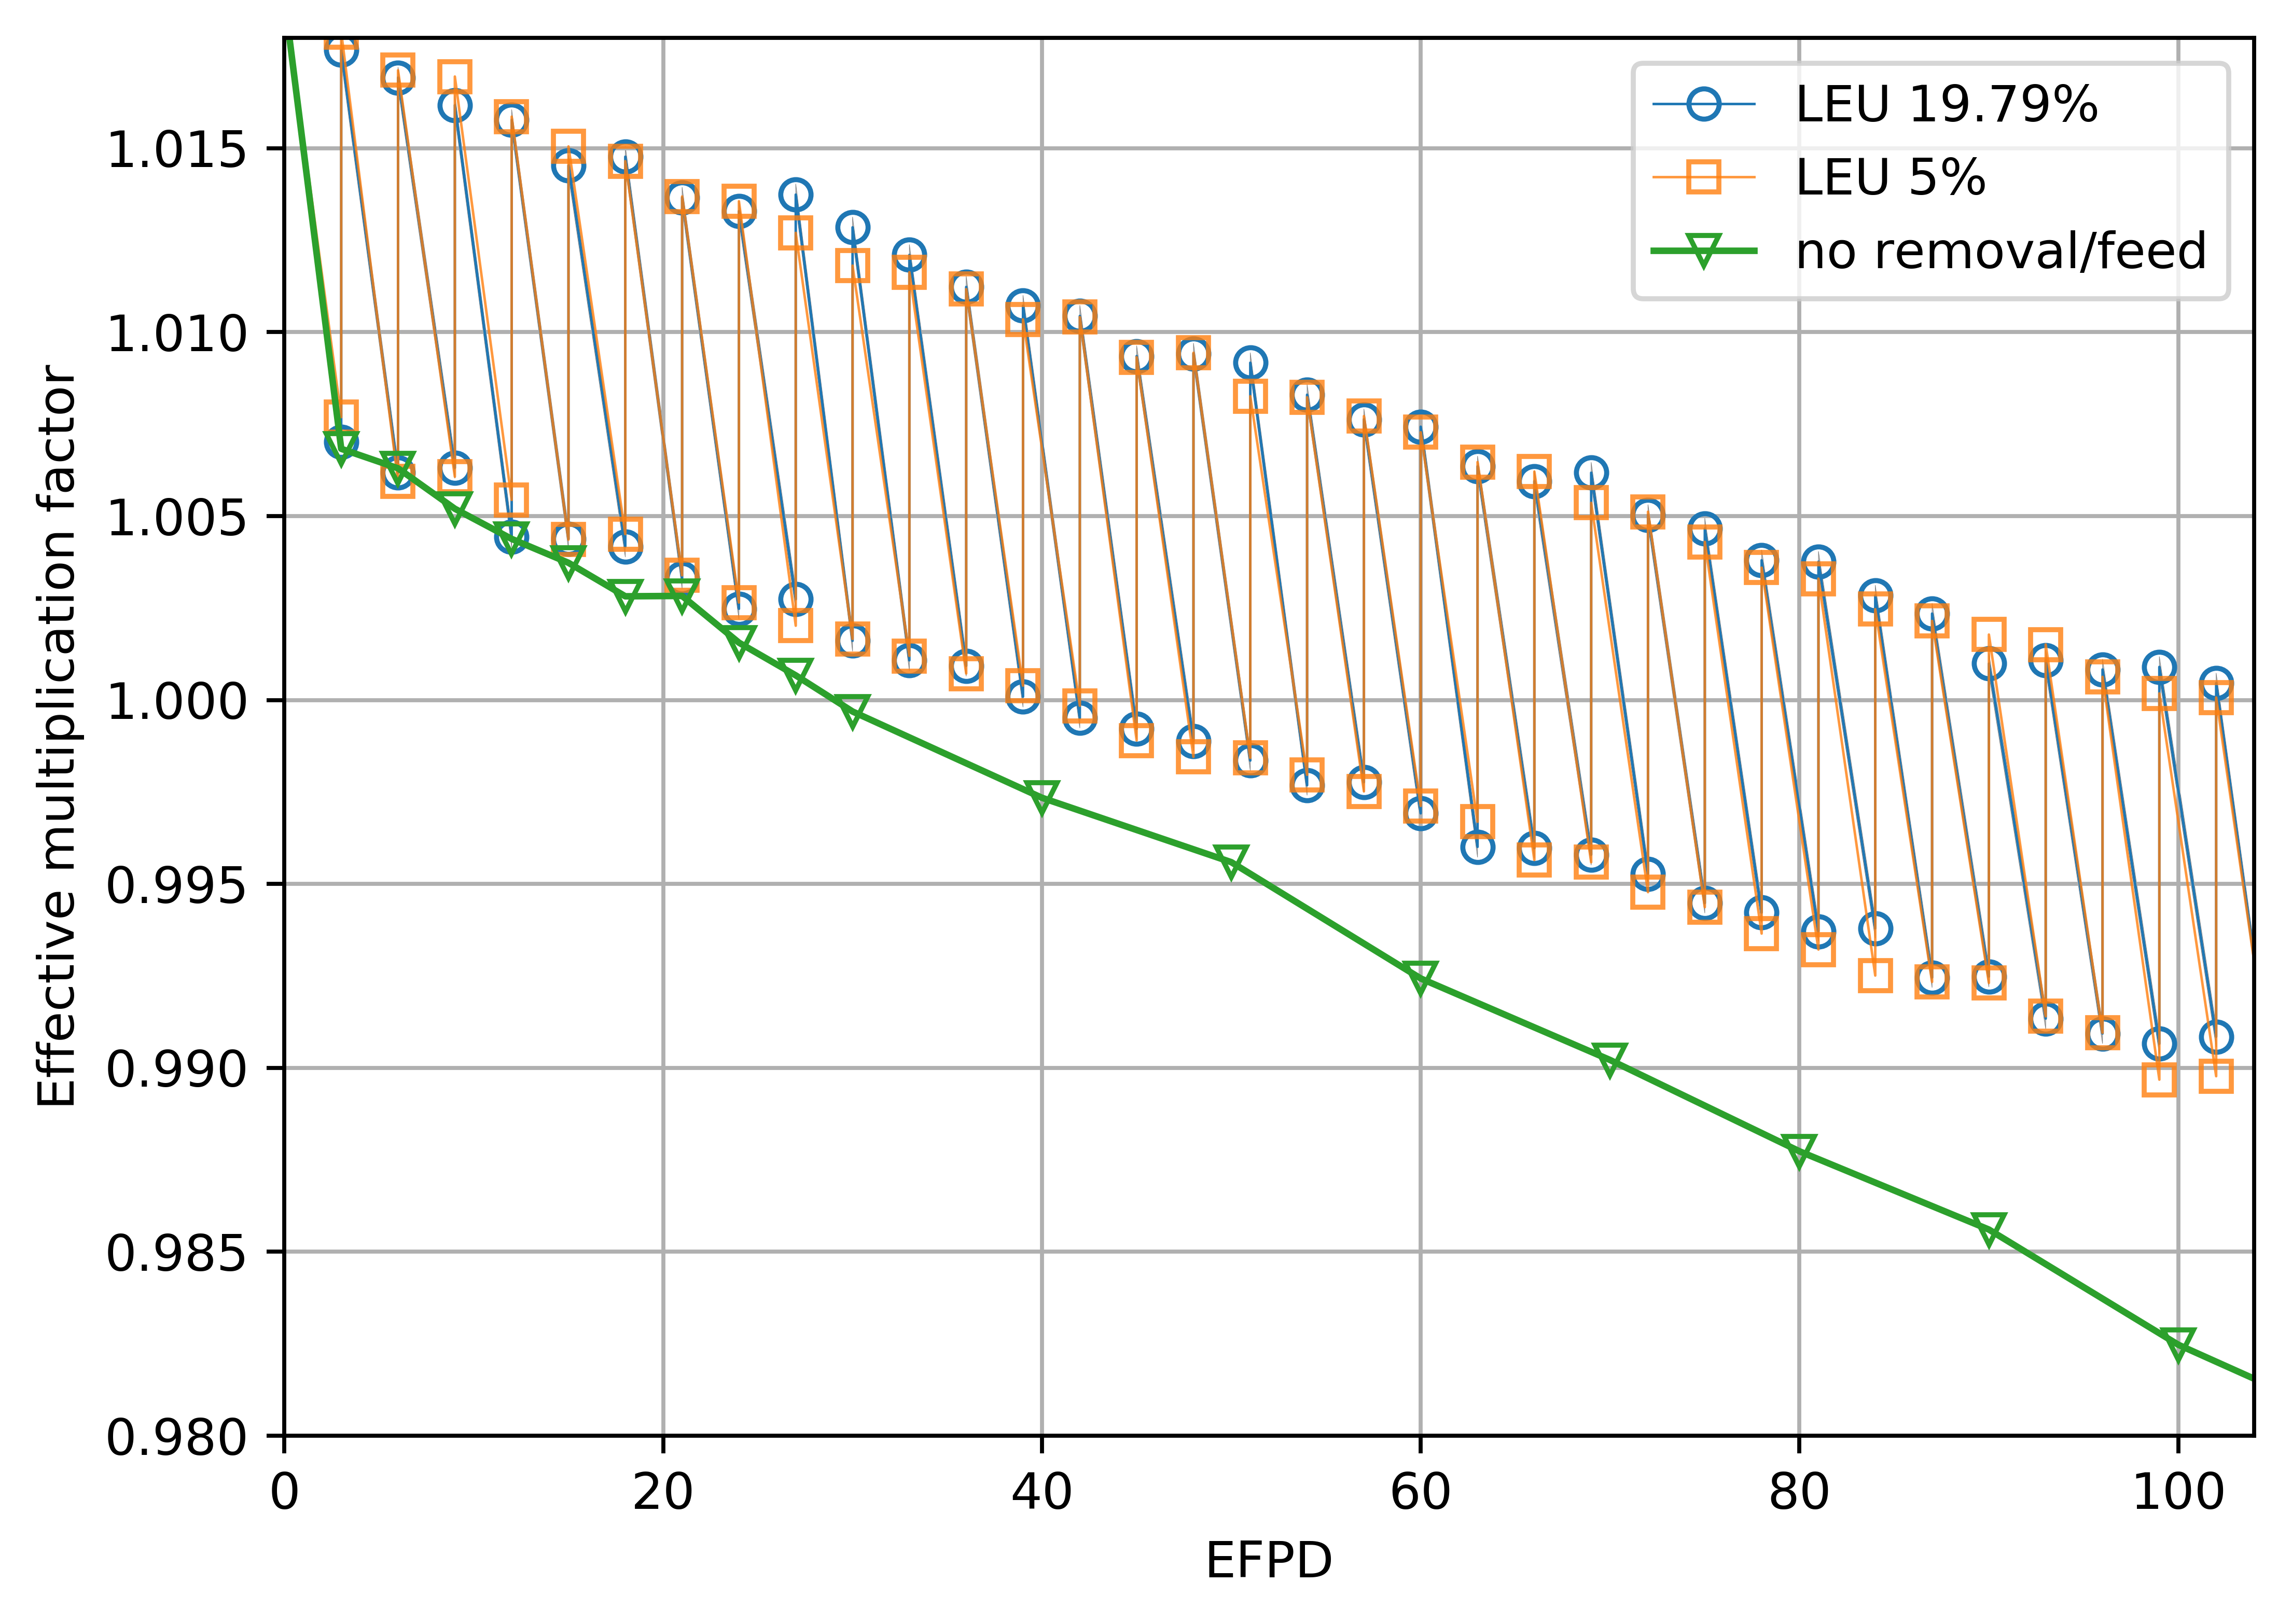
\includegraphics[width=0.85\textwidth]{keff_zoomed_1.png}
	  \vspace{-0.25in}
  \caption{Zoomed effective multiplication factor for the first 104 EFPD 
  after startup.}
  \label{fig:keff-zoomed}
\end{figure}
\begin{figure}[htp!] % replace 't' with 'b' to 
  \centering
		  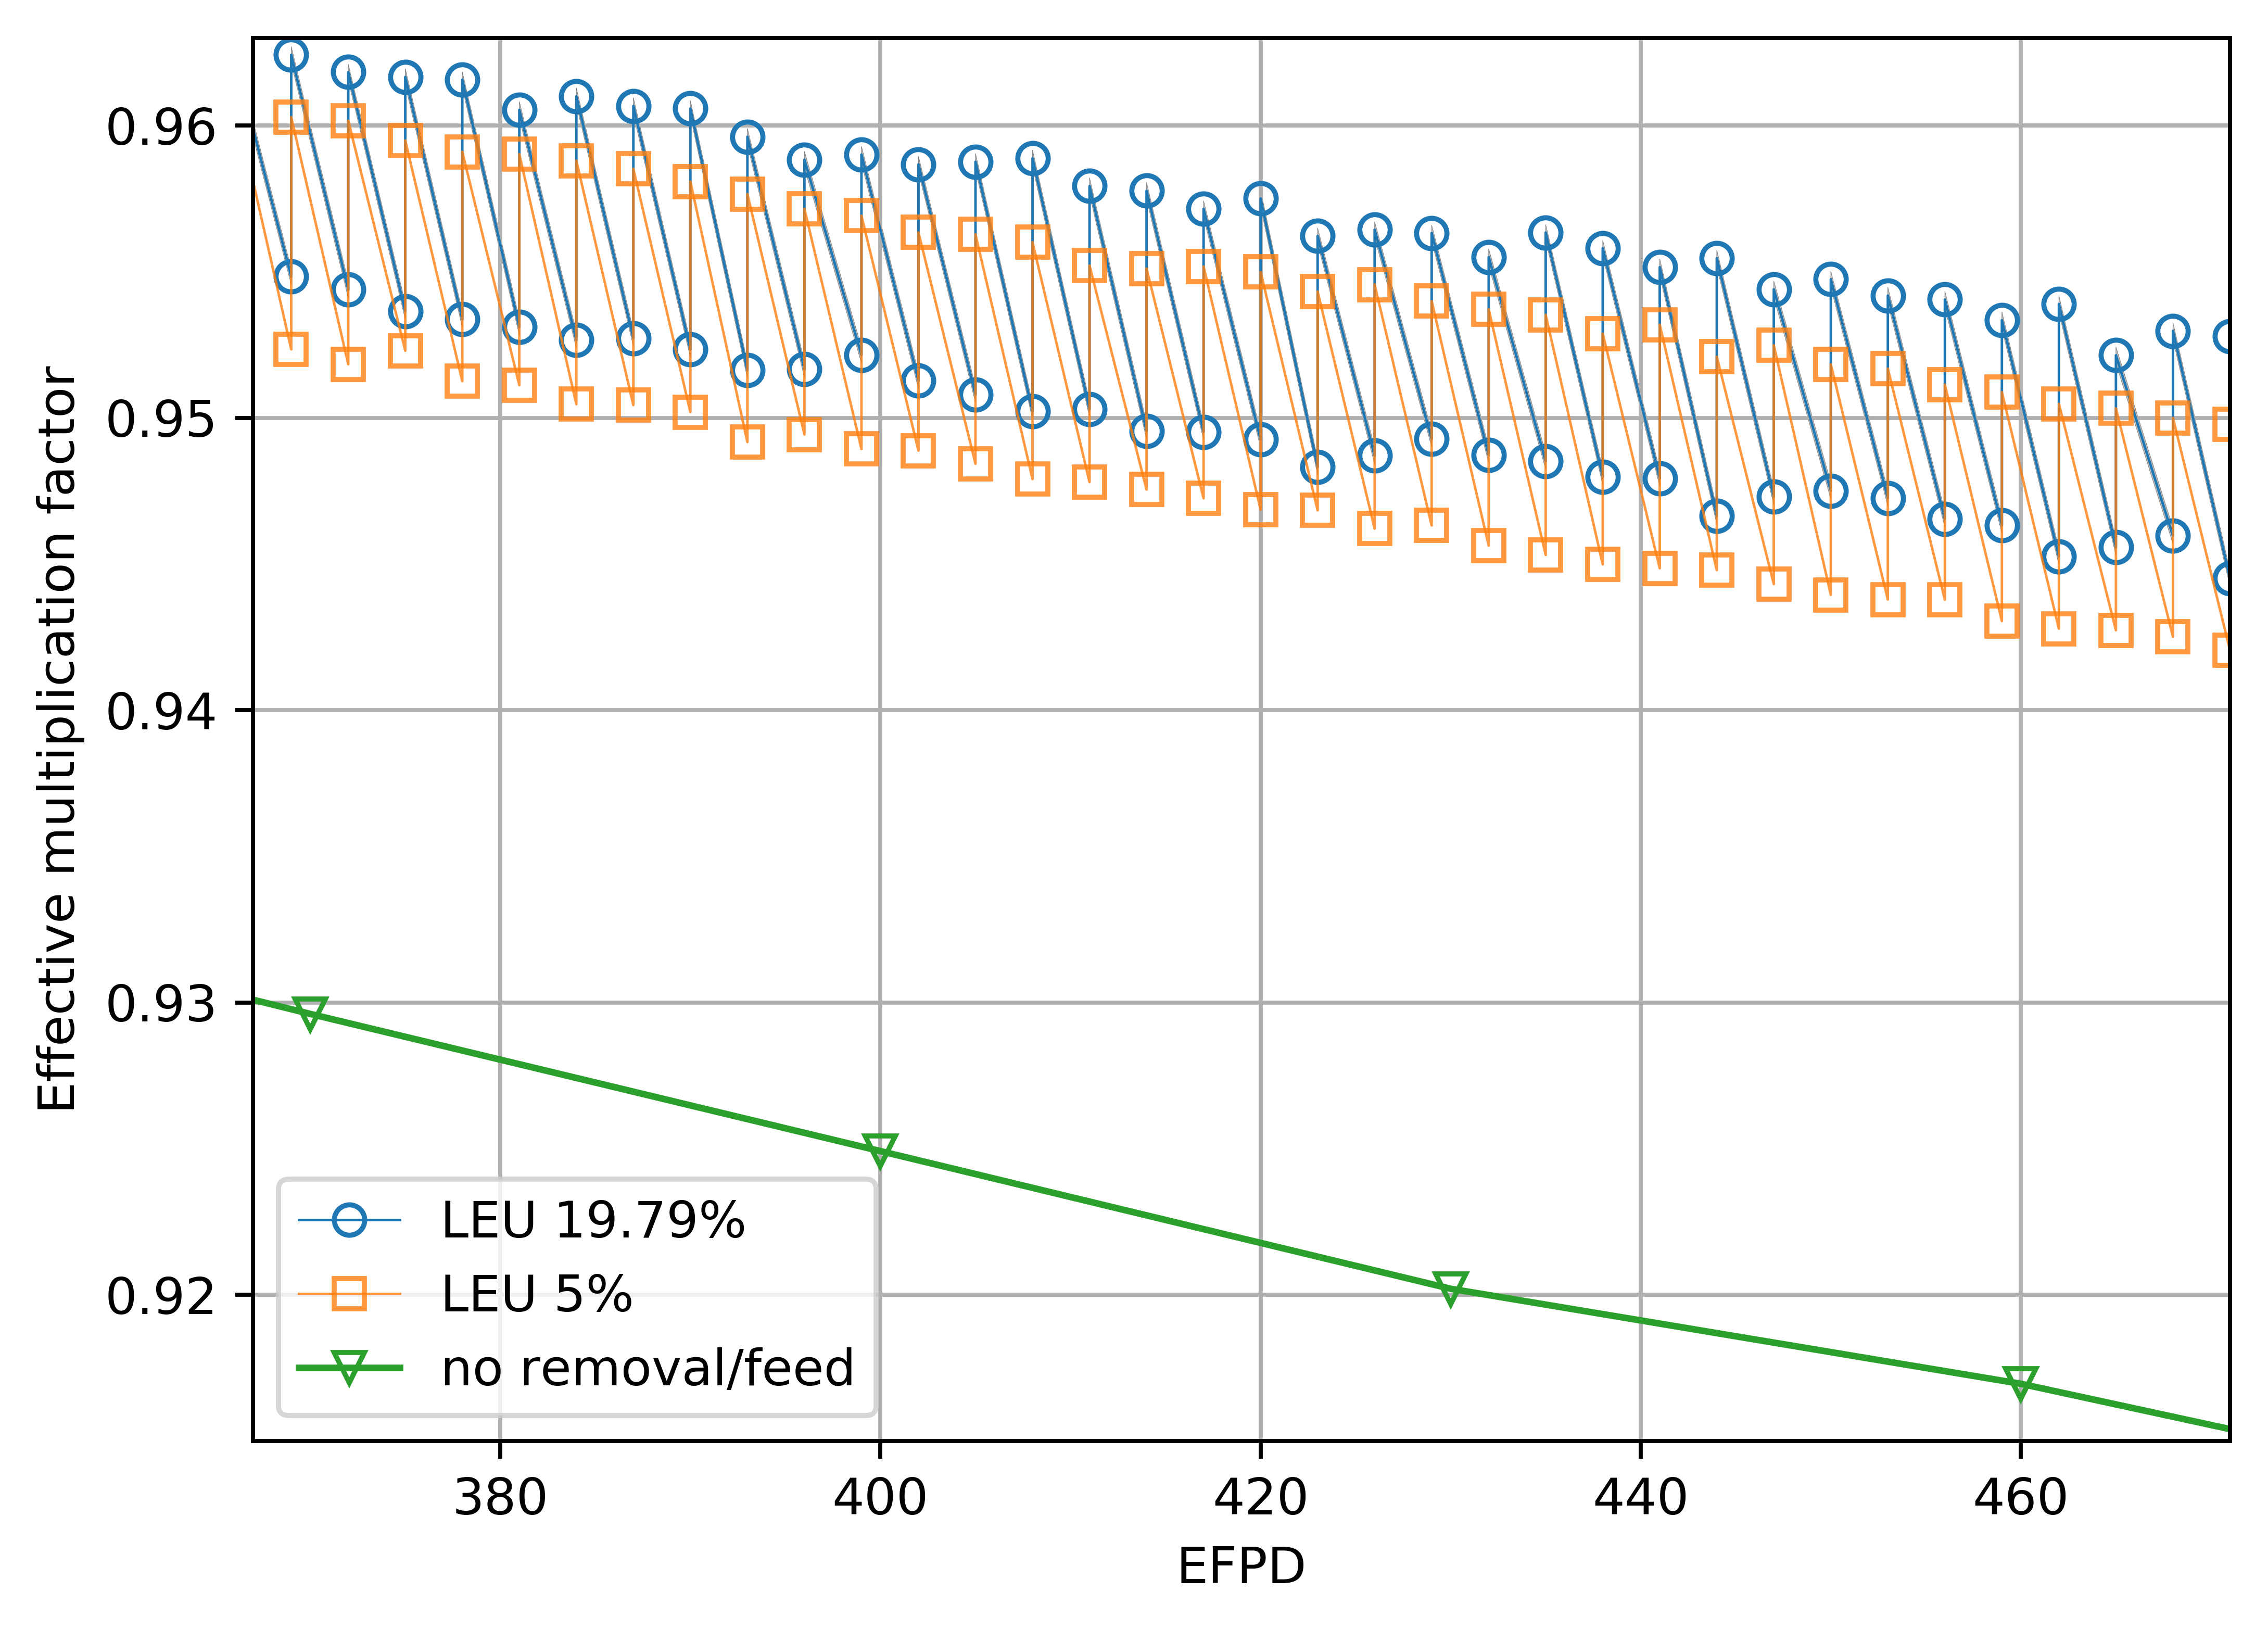
\includegraphics[width=0.85\textwidth]{keff_zoomed_2.png}
	 \vspace{-0.25in}
  \caption{Zoomed effective multiplication factor for the time interval 
  from 367 to 471 EFPD after startup.}
  \label{fig:keff-zoomed-2}
\end{figure}

Loading initial fuel salt composition with 5\% \gls{LEU} into the \gls{TAP} 
core leads to a supercritical configuration with an excess of reactivity about 
1900pcm (figure~\ref{fig:keff}). Without performing any fuel salt reprocessing 
the core became subcritical after 30 days of operation (figure~\ref{fig:keff-zoomed}). 
We obtained this result using naked Serpent without introducing any \gls{FP} extraction 
and refueling. For the beginning of the \gls{TAP} lifetime uranium enrichment in the 
feed has a minor effect because a tiny amount of poisons was produced (<1kg/day) and, 
hence, a small mass of fresh salt was injected. Notably, the core went subcritical after 
42 days of operation either with \gls{LEU} 5\% or \gls{LEU} 19.79\% feed.

The \gls{TAP} core is never reached equilibrium fuel salt composition without 
performing fuel salt reprocessing and refueling. For the fueling scenarios with 
5\% and 19.79\% \gls{LEU} feed, the reactor achieved the equilibrium state after 
11 and 10 years of operation, respectively. Overall, the effective multiplication 
factor gradually decreases from initial 1.018 to 0.88 for the 19.79\% 
\gls{LEU} feed and 0.86 for the 5\% \gls{LEU} feed, which indicates 
problems with operating this nuclear reactor design. We will try to overcome 
this issue by re-optimizing the \gls{TAP} core and design parameters as well as 
adding new functionality to SaltProc v2.0+.

Acting as a complement to Figure ~\ref{fig:keff}, the Figure~\ref{fig:shannon} 
shows Shannon entropy of a fission source as a function of the number of inactive 
cycles and clearly indicates that the Monte Carlo simulation convergences with a 
number of inactive cycles >200 \cite{brown_k-effective_2011-1}. 
\begin{figure}[htp!] % replace 't' with 'b' to 
  \centering
		  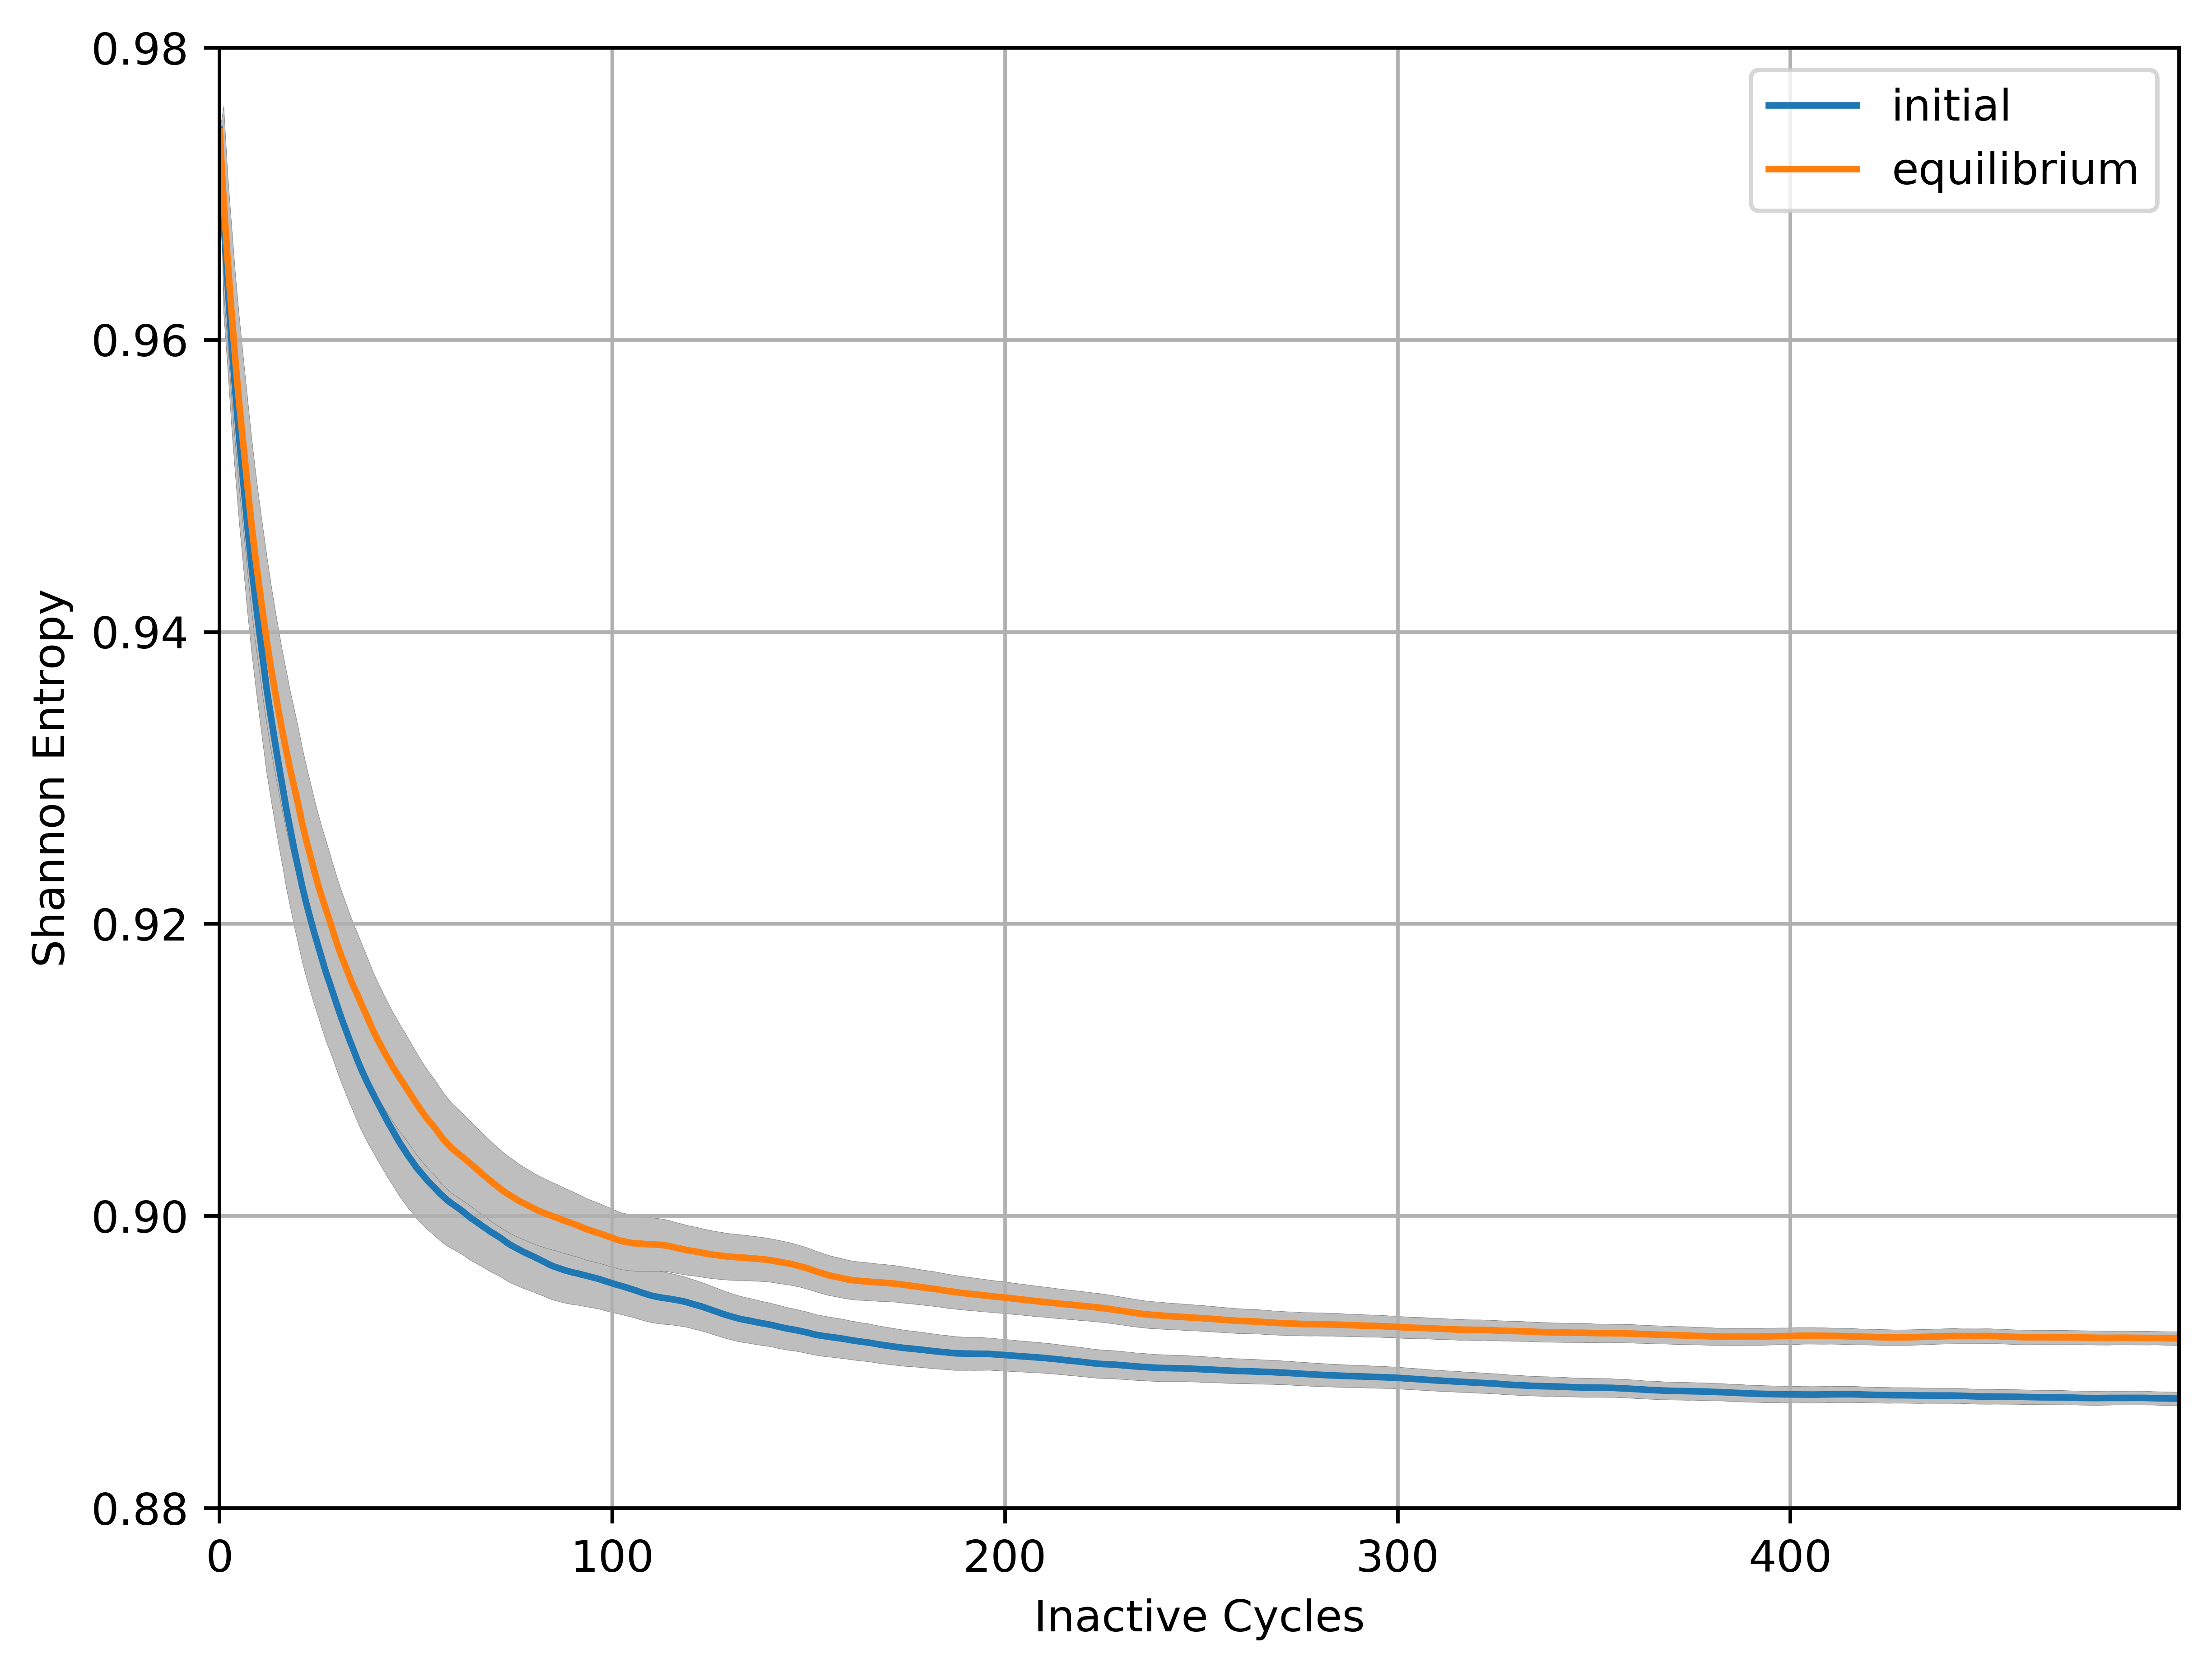
\includegraphics[width=\textwidth]{h_src.png}
	 \vspace{-0.35in}
  \caption{Shannon entropy of a fission source for initial and equilibrium 
  fuel salt composition as a function of inactive cycles number 
  for the full core calculations with neutron population $M=15'000$.}
  \label{fig:shannon}
\end{figure}

\subsection{Neutron spectrum}
Figure~\ref{fig:spectrum} shows the normalized neutron flux spectrum for the 
full-core \gls{TAP} core model in the energy range from 10$^{-8}$ to 15 MeV. 
The neutron energy spectrum at equilibrium is a little bit harder than at 
startup due to plutonium and other strong absorbers accumulating in the 
core during reactor operation. The \gls{TAP} spectrum is significantly 
harder than in a typical \gls{LWR} and is in a good agreement with 
\gls{ORNL} report \cite{betzler_assessment_2017}.
\begin{figure}[htp!] % replace 't' with 'b' to 
  \centering
		  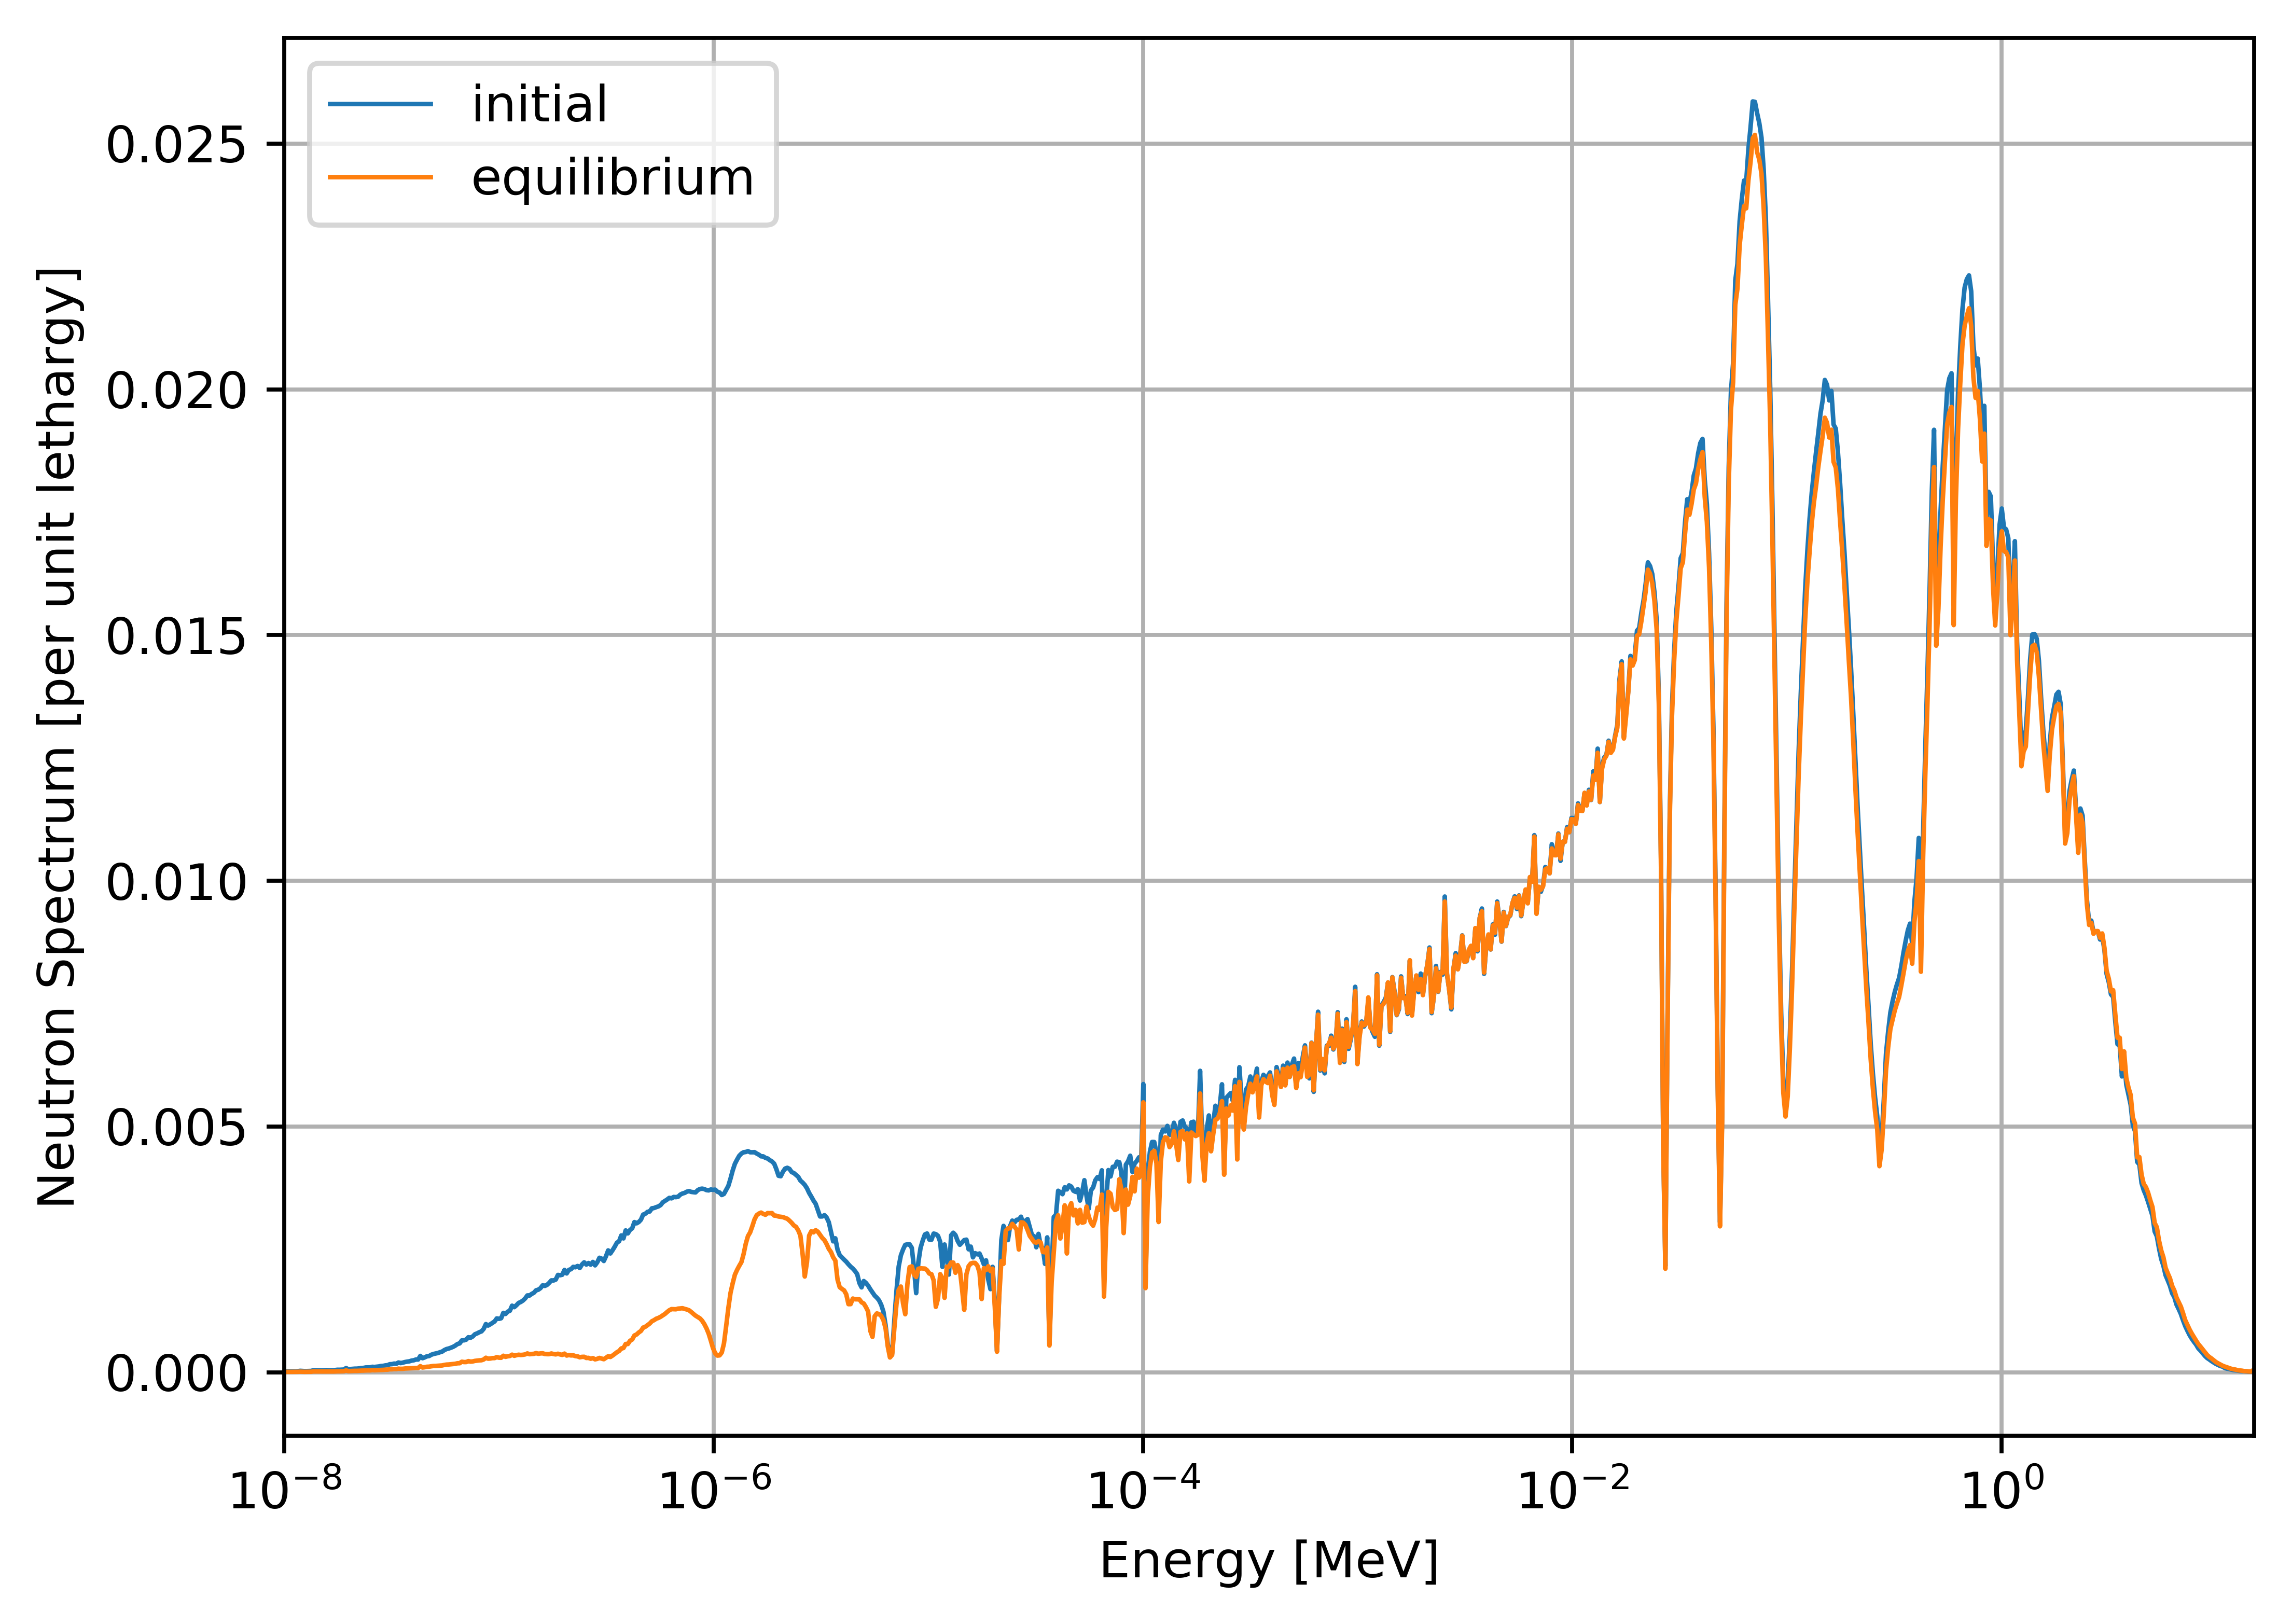
\includegraphics[width=\textwidth]{spectrum.png}
	 \vspace{-0.35in}
  \caption{The neutron flux energy spectrum normalized by unit lethargy 
  for initial and equilibrium fuel 
  salt composition for 5\% and 19.79\% \gls{LEU} feed.}
  \label{fig:spectrum}
\end{figure}
\section{Fuel salt composition}
Figure~\ref{fig:u-pu} shows the absolute mass of major heavy isotopes 
which have a strong influence on the reactor core physics. The mass of 
$^{236}$U, $^{238}$U, $^{239}$Pu, $^{240}$Pu, and $^{241}$Pu in the 
fuel salt changes insignificantly after approximately 10 years of operation,
which matches stabilization time for effective multiplication factor. 
Hence, the quasi-equilibrium state was reached after 10 years of reactor 
operation. Moreover, the \gls{TAP} core bred approximately the same amount 
of fissile $^{239}$Pu ($\approx2$t) as was initial fissile material 
($^{235}$U) load. A significant amount of non-fissile plutonium builds 
up during operation and accounts for 50\% of the plutonium after 13 years 
of operation. Overall, rate of breeding fissile $^{239}$Pu from $^{238}$U 
even in relatively hard neutron spectrum is not large enough to compensate 
negative effects of strong absorbers accumulation and keep the reactor 
critical.
\begin{figure}[htp!] % replace 't' with 'b' to 
  \centering
		  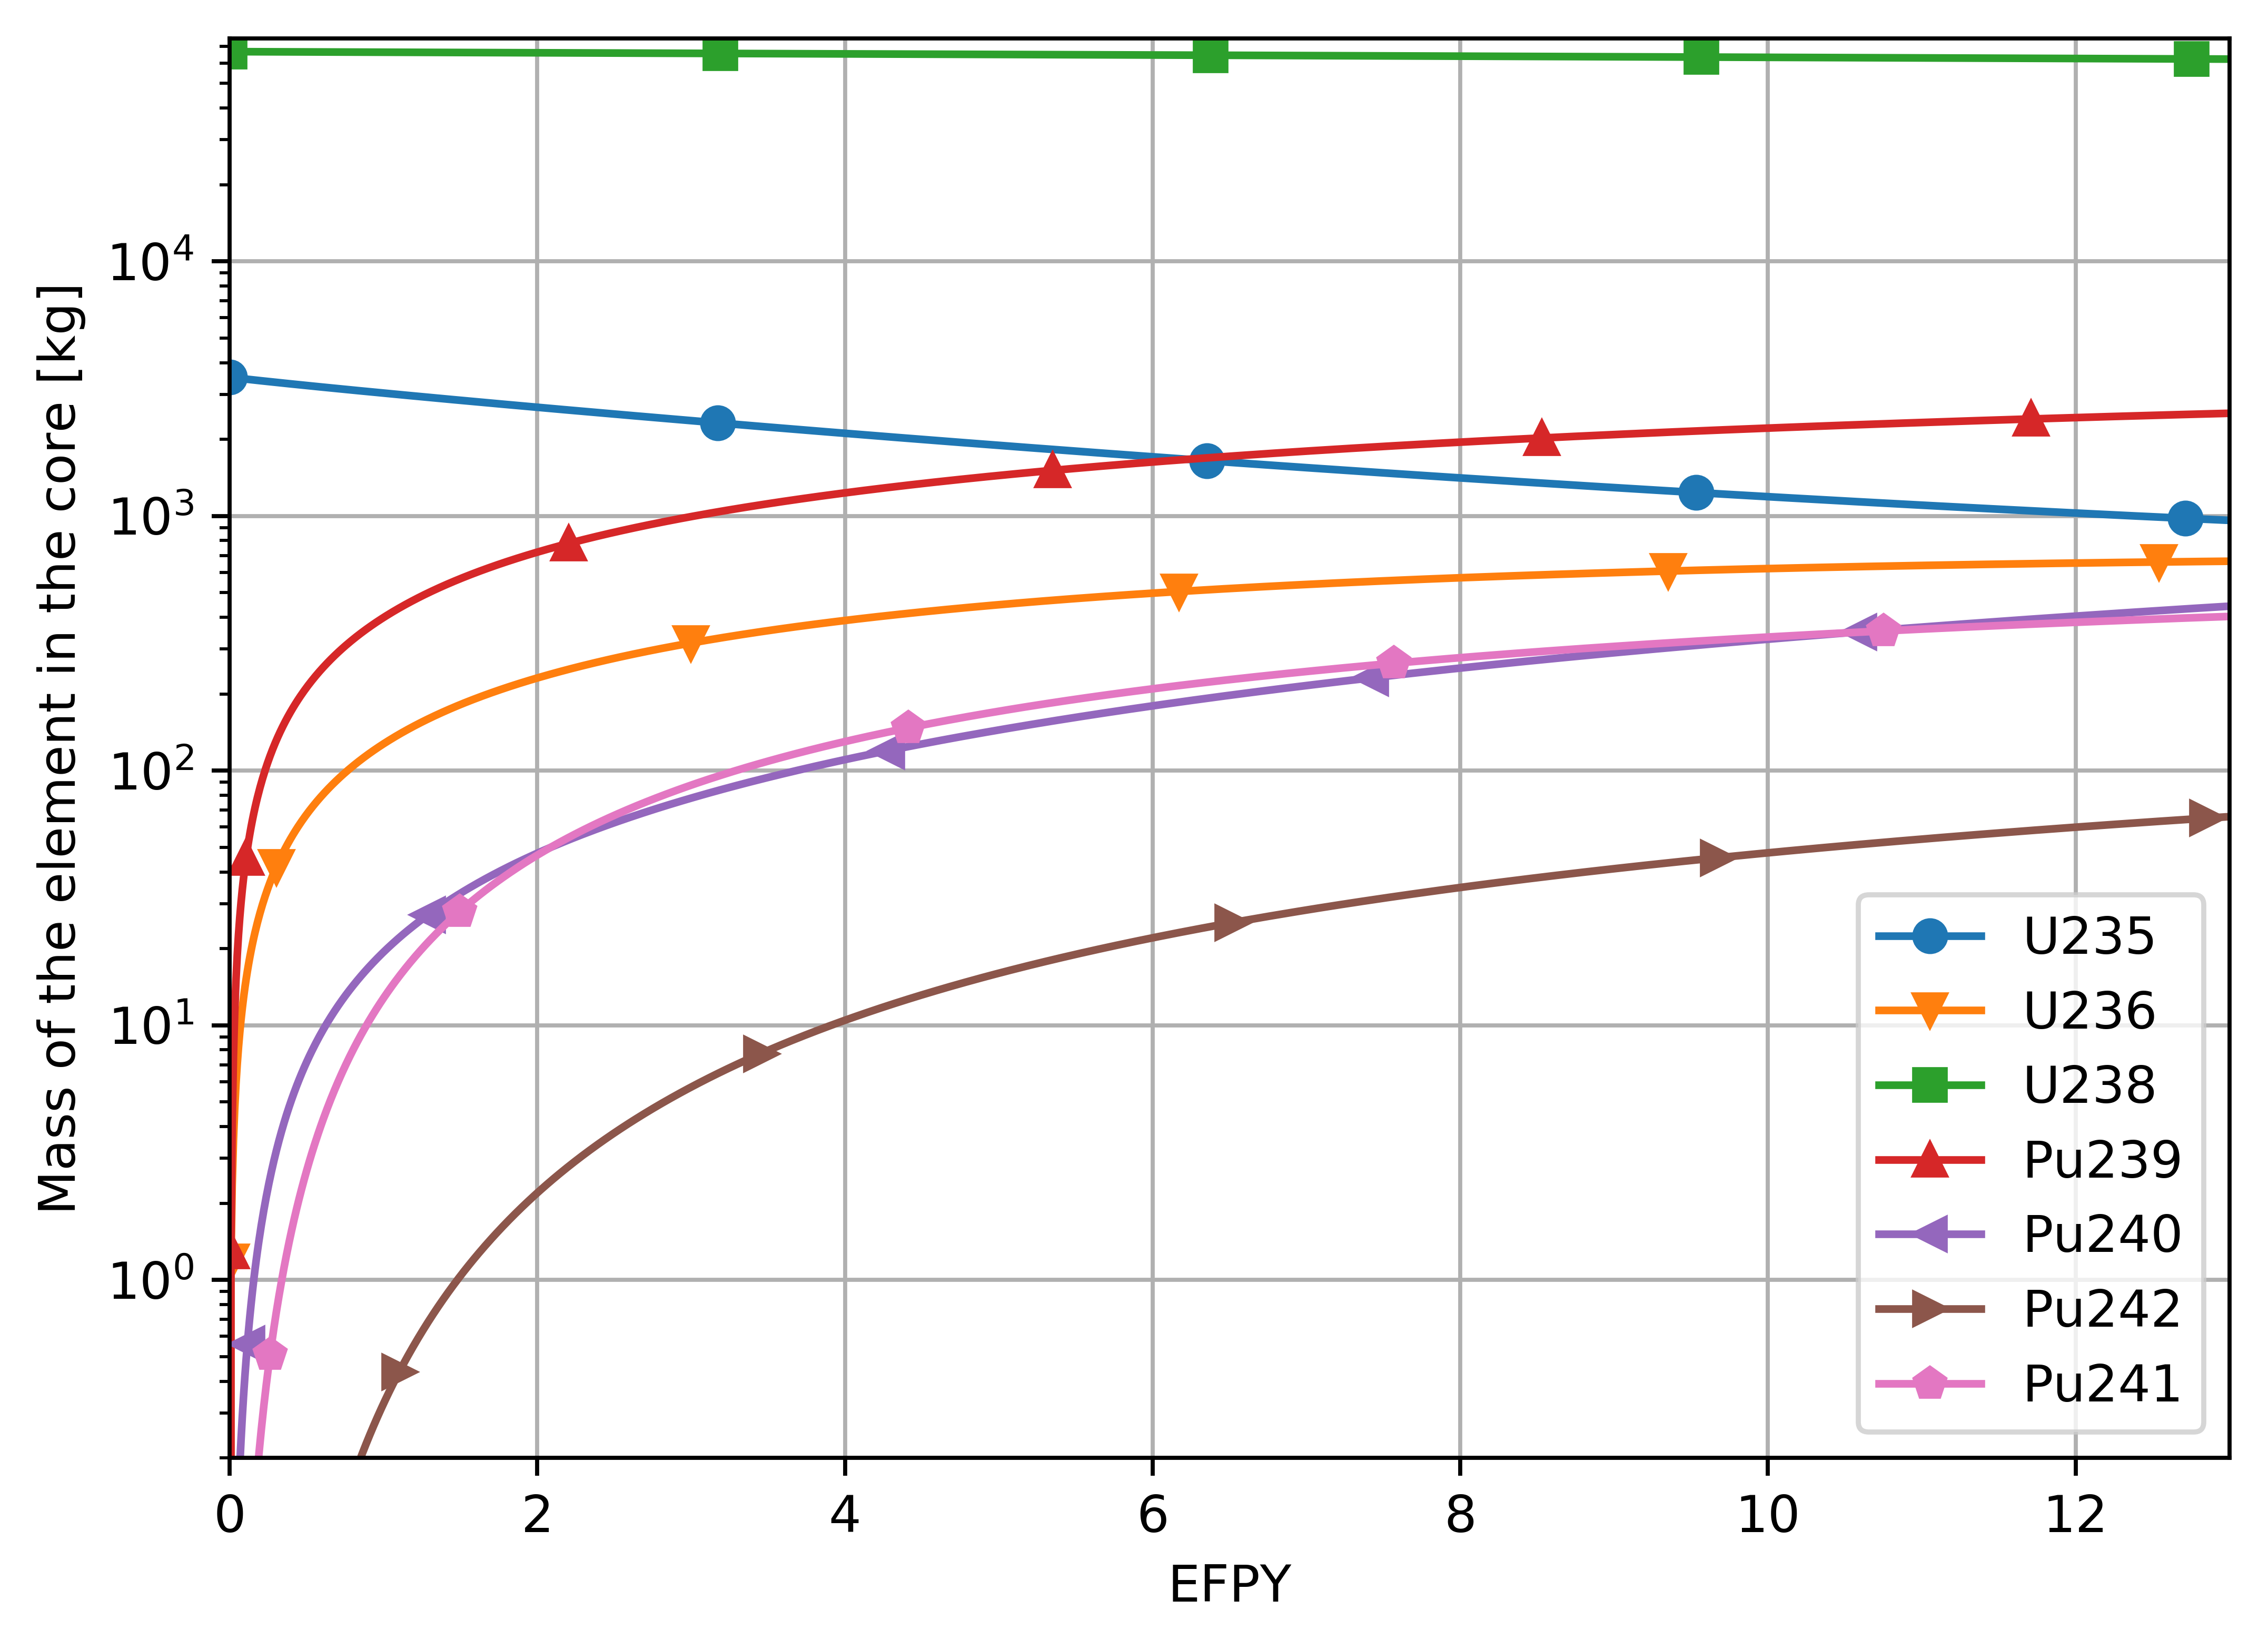
\includegraphics[width=1.03\textwidth]{u_pu_mass.png}
	 \vspace{-0.4in}
  \caption{Mass of major nuclides during 13 years of reactor operation 
  with 19.79\% \gls{LEU} feed.}
  \label{fig:u-pu}
\end{figure}

We checked correctness of SaltProc v2.0+ by comparing mass of important 
for load-following operation isotopes ($^{135}$Xe, $^{135}$I) to expected 
mass after each depletion step (figure~\ref{fig:xe-i}). For $^{135}$Xe 
expected mass was calculated as follows:
\begin{align}
& m_{after\;reprocessing} = m_{before\;reprocessing} \times  \epsilon_{sparger} \times \epsilon_{separator}
	\intertext{where}
 	m_{after} &= \mbox{the mass of the isotope after applying removals and feeds} \nonumber \\
 	m_{before} &= \mbox{the mass of the isotope right before  reprocessing} \nonumber \\
 	\epsilon_{sparger} &= \mbox{the sparger extraction efficiency} \nonumber \\
 	\epsilon_{separator} &= \mbox{the entrainment separator extraction efficiency} \nonumber
\end{align}
\begin{figure}[htp!] % replace 't' with 'b' to 
  \centering
		  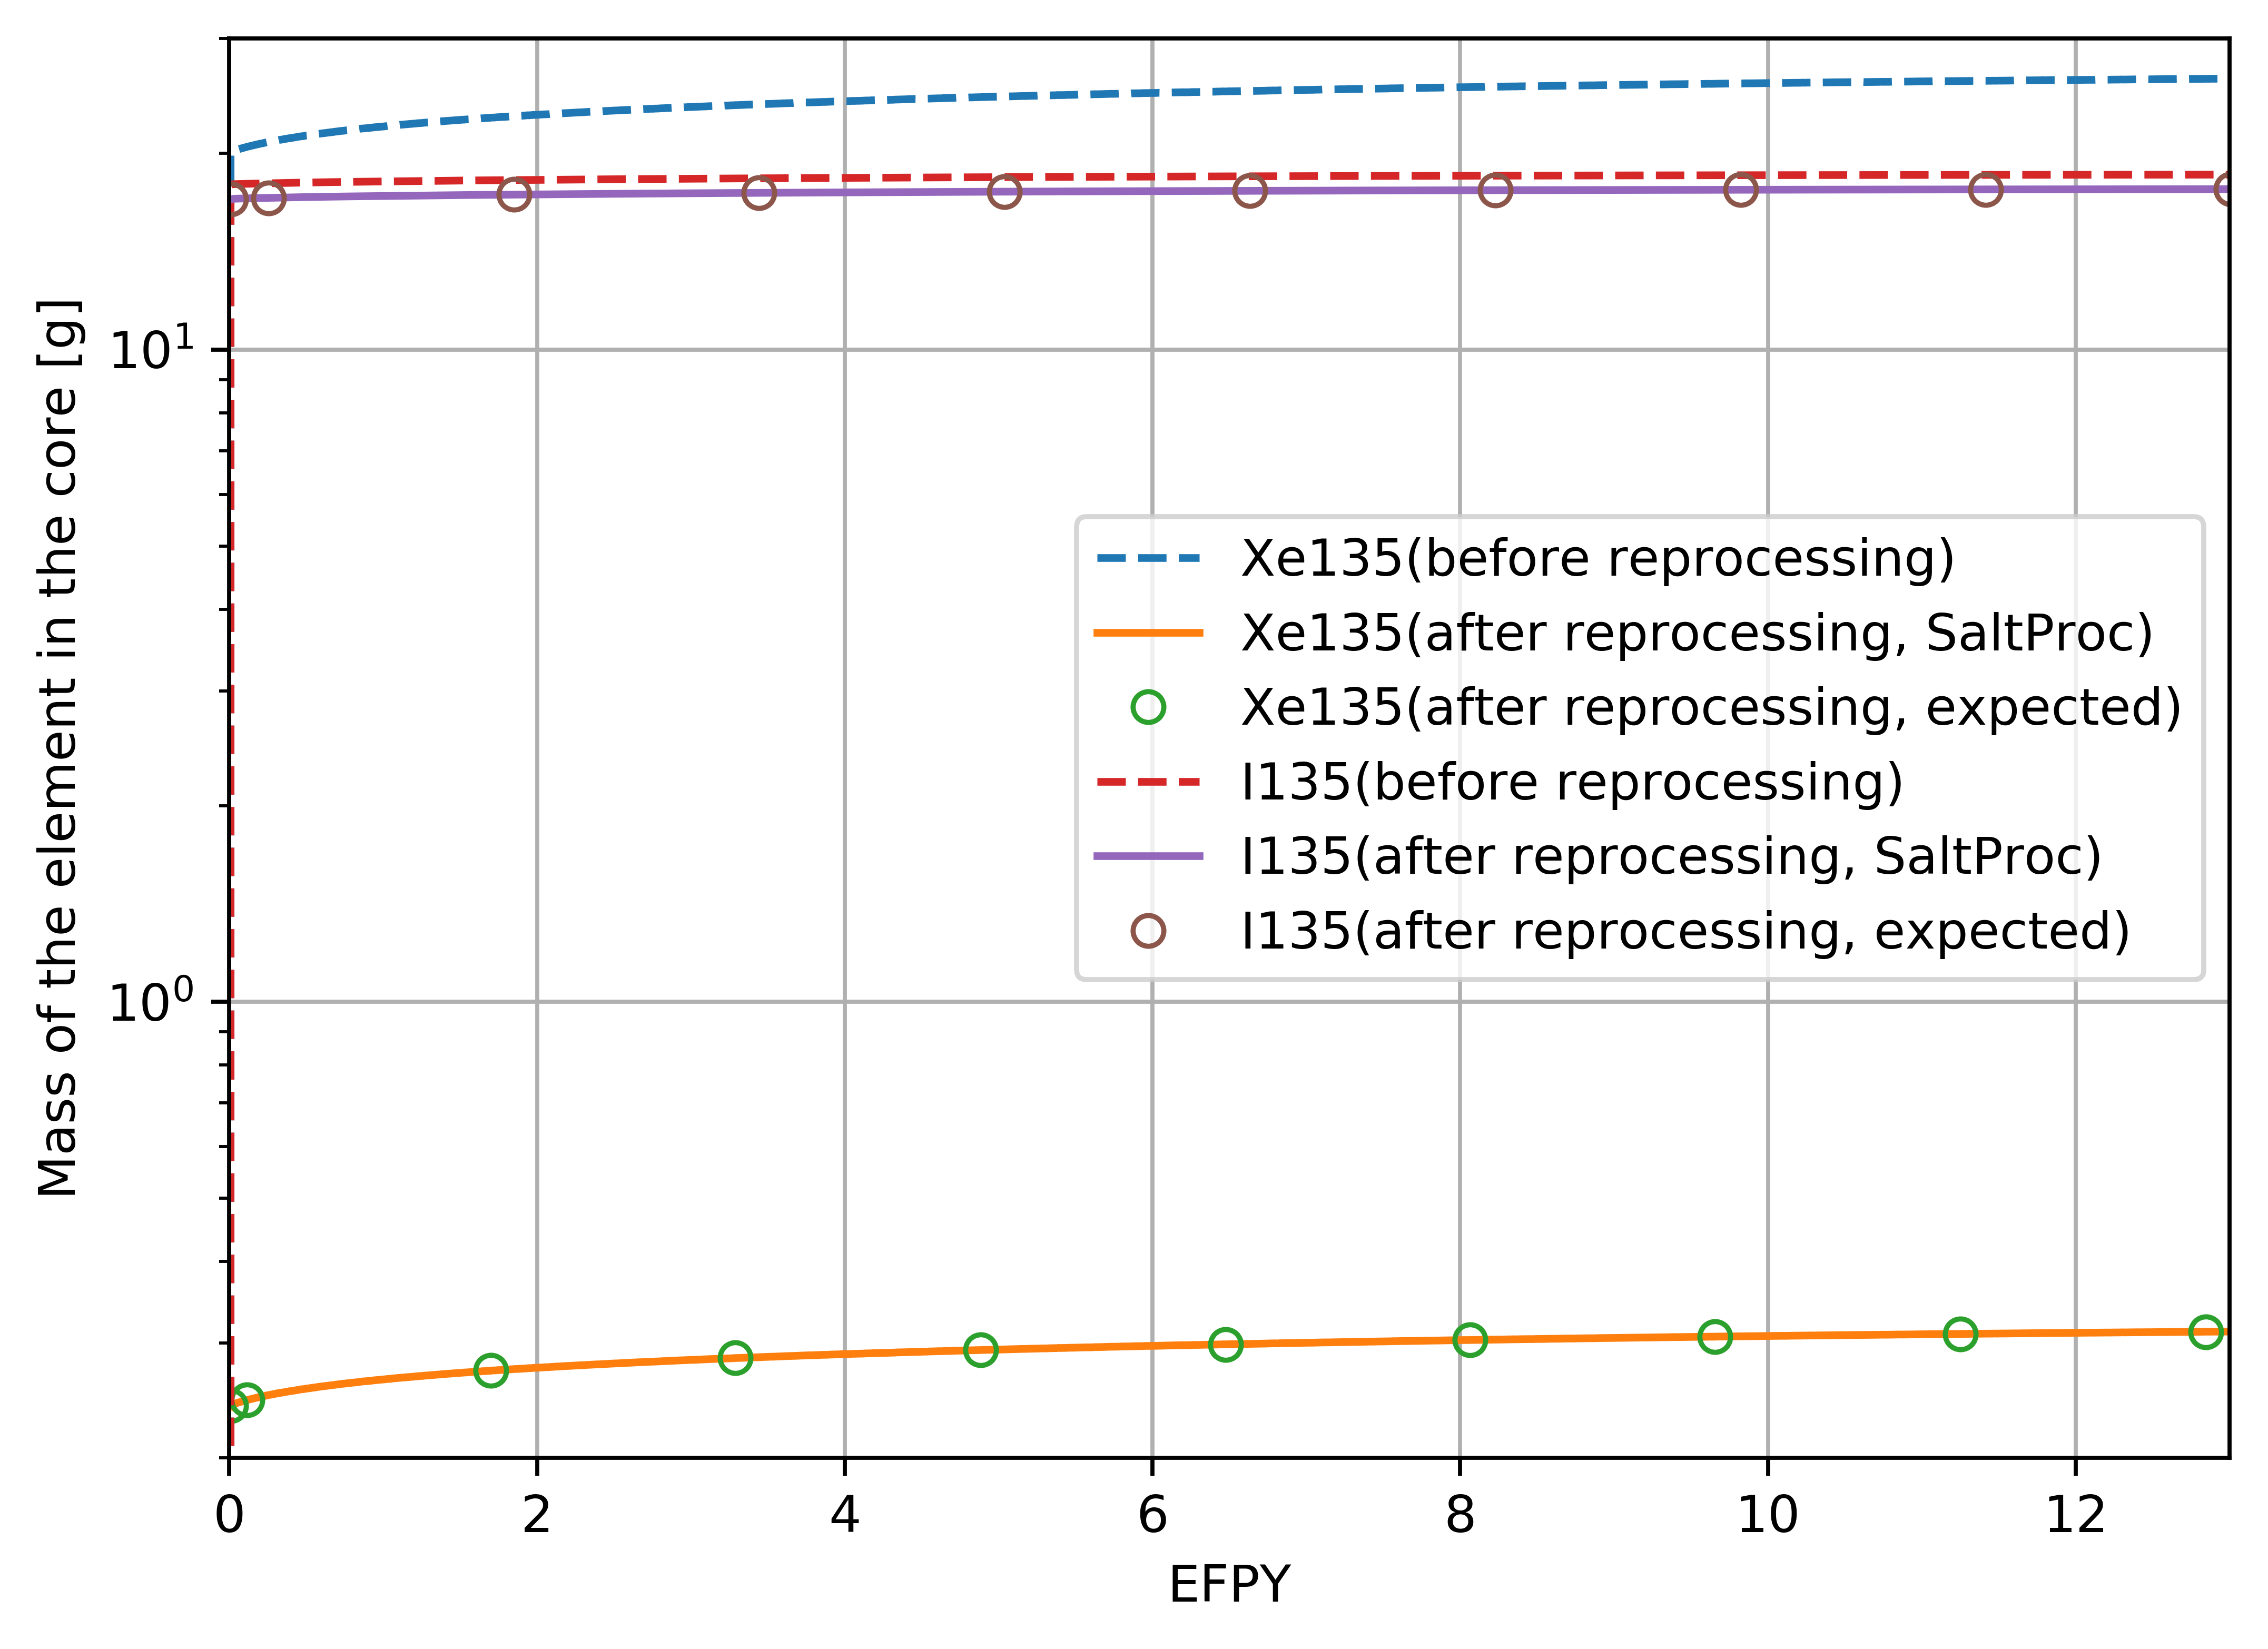
\includegraphics[width=\textwidth]{xe_i_mass.png}
	 \vspace{-0.35in}
  \caption{Mass of major neutron poison, $^{135}$Xe, and its main precursor, 
   $^{135}$I, during 13 years of reactor operation before and after reprocessing.}
  \label{fig:xe-i}
\end{figure}

For the iodine approach is similar, but the extraction efficiency of iodine in the nickel 
filter is only 5\%. Figure~\ref{fig:xe-i} shows that SaltProc v2.0+ extraction module 
correctly removes target isotopes with specified extraction efficiency: 
SaltProc and expected mass match. Overall, the \gls{TAP} fuel reprocessing 
system simulated with SaltProc v2.0+ allows keeping $^{135}$Xe inventory in the core 
during operation on 100\% power as low as 1g.
\section{Future work}
The \gls{TAP} core should be able to maintain a critical state ($k_{eff}\geq 1.0$) 
for at least 30 years of operation lifetime. We will re-optimize and improve the 
\gls{TAP} reactor model by performing the next steps:
\paragraph{$k$ eigenvalue at \gls{BOL}:} The effective multiplication factor is 
too small at the \gls{BOL}. The most recent 
\gls{ORNL} paper \cite{betzler_fuel_2018} reported initial $k$ eigenvalue calculated 
for \gls{BOL} about 1.035 which is much greater than our result 
($1.01909\pm23pcm$). We will reduce fast neutron leakage by adding an appropriate 
reflector and thermal insulation around the vessel to get a larger excess of 
reactivity at the \gls{BOL}.
\paragraph{Dynamic moderator-to-volume fraction:} The \gls{TAP} major feature is 
the ability to adjust moderator-to-volume, or \gls{SVF}, ratio during lifetime 
by changing moderator rods configuration. Adding more moderator in the core 
thermalizes neutron spectrum and significantly extends the core lifetime. 
Unfortunately, the \gls{TAP} White 
papers and \gls{ORNL} technical reports lack details about how those configurations 
are formed. 
We will create various geometries with various \gls{SVF} based on assumption, 
that the plant personnel is reconfiguring the
moderator rods only at regular intervals (i.e., 18 months) during the shutdown for 
reactor maintenance. That is, we assuming that the reactor maintaining
the long-term reactivity by periodically replacing stationary
zirconium hydride rod assemblies with those containing more rods
(e.g., replacement of a four-rod assembly with a nine-rod assembly) 
\cite{betzler_fuel_2018}. 
Additionally, we will add in SaltProc v2.0+ capability to switch from one 
geometry file to another with a user-defined time interval. 
\paragraph{Reprocessing scheme:} Extraction efficiencies and refueling strategy 
of the \gls{TAP} fuel reprocessing and refueling plant will be revised to make 
sure that all possible strong poisons are removed with an appropriate rate.

\bibliographystyle{ieeetr}
\bibliography{q4-report}

%\bibliographystyle{plain}

%\printbibliography

\end{document}
